\documentclass[11pt, ngerman, fleqn, DIV=15, headinclude, BCOR=2cm]{scrreprt}

\usepackage{../../header}

\usepackage[section]{placeins}
\usepackage[maxfloats=50]{morefloats}

\usepackage{csquotes}
\usepackage{fancyvrb}
\usepackage{../pygments}

\usepackage{pdflscape}

\usepackage{tikz}
\usetikzlibrary{chains}
\usetikzlibrary{shapes.geometric}

\tikzset{device/.style={
        rectangle,
        minimum size=6mm,
        draw=black
    },
    monitor/.style={
        rectangle,
        rounded corners=2mm,
        minimum size=6mm,
        draw=black
    },
}

\def\table{\def\figurename{Tabelle}\figure}
\let\endtable\endfigure

\usepackage{pgfplots}
\pgfplotsset{
    compat=1.9,
    width=0.8\linewidth,
    xticklabel style={/pgf/number format/use comma},
    yticklabel style={/pgf/number format/use comma},
}
\usepgfplotslibrary{polar}

\usepgfplotslibrary{external}
\tikzexternalize[mode=list and make]
\tikzsetexternalprefix{Abbildung-}

\DeclareSIUnit{\skt}{SKT}

\usepackage{booktabs}

\hypersetup{
    pdftitle=
}

\subject{Praktikumsprotokoll}
\title{Höhenstrahlung}
\subtitle{Versuch P518 -- Universität Bonn}
\author{
    Martin Ueding \\
    \small{\href{mailto:mu@martin-ueding.de}{mu@martin-ueding.de}}
    \and
    Lino Lemmer \\
    \small{\href{mailto:l2@uni-bonn.de}{l2@uni-bonn.de}}
}

\date{\daterange{2014-07-02}{2014-07-03}}

\publishers{Tutor: Michael Lupberger}

\begin{document}

\maketitle

\begin{abstract}
    Wir vermessen die Energie- und Winkelabhängigkeit der Höhenstrahlung.
    Außerdem bestimmen wir die Lebensdauer der Myonen.
\end{abstract}

\tableofcontents

\chapter{Theorie}

\section{Höhenstrahlung}

Deutlich außerhalb der Atmosphäre befinden sich hochenergetische Teilchen, die
beim Eintritt in die Atmosphäre diverse Reaktionen verursachen.

Die Primärstrahlung besteht zum Großteil aus Protonen und hat Energien bis
\SI{e21}{\electronvolt}, der Mittelwert liegt im Bereich
\SIrange{e9}{e10}{\electronvolt} \parencite[983]{meschede-gerthsen_24}. Der
Anteil der Protonen ist ungefähr \SI{85}{\percent}
\parencite[110]{Grupen/Astroteilchenphysik}.

Diese teils sehr harten Teilchen zerfallen in der Atmosphäre in verschiedene
Leptonen, Photonen und Mesonen. Dabei treten folgende Zerfälle auf, die Myonen
erzeugen \parencite[111]{Grupen/Astroteilchenphysik}:

\label{sec:muon-channels}
\begin{itemize}
    \item
        $\piup^+ \to \muup^+ + \nuup_\muup$
    \item
        $\piup^- \to \muup^- + \bar \nuup_\muup$
    \item
        $\mathrm K^+ \to \muup^+ + \nuup_\muup$
    \item
        $\mathrm K^- \to \muup^- + \bar \nuup_\muup$
\end{itemize}

Da Pionen eine geringe Ruhemasse haben, werden sie in großer Anzahl in
Hadronenschauern erzeugt. Sie zerfallen schnell – Lebensdauer von
\SI{26}{\nano\second} \parencite[111]{Grupen/Astroteilchenphysik} – und
erzeugen so viele Myonen. Daher folgt das Energiespektrum der Myonen dem der
Pionen \parencite[113]{Grupen/Astroteilchenphysik}.

Myonen haben eine hohe Ruhemasse und verlieren
daher wenig Energie durch Bremsstrahlung. Daher kommen Sie hochenergetisch an
der Erdoberfläche an \parencite[984]{meschede-gerthsen_24}. Sie stellen einen
Anteil von \SI{80}{\percent} der geladenen Teilchen, die bis auf die
Erdoberfläche durchdringen \parencite[111]{Grupen/Astroteilchenphysik}.

Diese Myonen sind die Teilchen, die wir hier im Versuch untersuchen werden.

Die Winkelabhängigkeit der Myonen ist, wenn man die Ablenkung durch das
Erdmagnetfeld ignoriert, isotrop in der Azimutrichtung und ungefähr
$\cos(\theta)^2$ in der Höhe \parencite[(7.2)]{Grupen/Astroteilchenphysik}.
Diese Verteilung ist in Abbildung~\ref{fig:cos2} skizziert. Die
\emph{atmosphärische Tiefe}, also die Menge an Materie in der Luftsäule über
dem Detektor, steigt mit dem Winkel zum Zenit. Daher gibt es mehr Möglichkeiten
für die Erzeugung der Myonen. Jedoch wird der Hauptteil des Flusses durch
weniger energetische Myonen ausgemacht. Diese haben auf dem größeren Weg mehr
Zerfallsmöglichkeiten in zum Beispiel Elektronen.
\parencite[115]{Grupen/Astroteilchenphysik}

\begin{figure}[htbp]
    \centering
    \tikzsetnextfilename{cos2}
    \begin{tikzpicture}
        \begin{polaraxis}
            \addplot[black] table {cos2.csv};
        \end{polaraxis}
    \end{tikzpicture}
    \caption{%
        Erwartete Intensitätsverteilung der Höhenstrahlung $\cos(\theta)^2$.
        Dabei ist $\theta$ hier so gewählt, dass $\theta = \SI{0}{\degree}$
        einer Einstrahlung senkrecht zum Erdboden entspricht.
    }
    \label{fig:cos2}
\end{figure}

\section{Standardmodell}

\subsection{Protonen und Neutronen}

Proton und Neutron sind Hadronen, die aus up- und down-Quarks zusammengesetzt
sind. Sie haben beide Spin $S$ und Isospin $I$ von $\frac12$. Sie unterscheiden
sich in der $I_3$-Komponente, dort hat das Proton $\frac12$, das Neutron
$-\frac12$.

Über das $W^-$-Boson, einem Vermittler der schwachen Wechselwirkung, kann das
Neutron in ein Proton zerfallen:
\[
    \mathrm n \to \mathrm p + \mathrm e^- + \bar
    \nuup_\mathrm e
    \iff
    \mathrm d
    \to
    \mathrm u + \mathrm W^-
    \to
    \mathrm u
    + \mathrm e^- + \bar \nuup_\mathrm e
\]

Das Proton ist stabil, das Neutron zerfällt jedoch innerhalb Minuten.

\subsection{Photonen}

Photonen sind die Vermittler der elektromagnetischen Wechselwirkung. Sie sind
masselos und tragen keinerlei Ladung. Sie haben jedoch Spin $S = 1$ und können
positive und negative Helizität haben, können also polarisiert sein. Die
Energie eines Photons ist $\hbar \omega$.

Steht ein weiteres Teilchen als Stoßpartner zur Verfügung, so erlaubt es die
Energie- und Impulserhaltung, dass ein Photon ein Teilchen-Antiteilchen-Paar
erzeugt (Paarbildung).

\subsection{Elektronen, Myonen, Neutrinos}

Elektronen und Myonen (sowie das Tau) sind die drei Familien von Leptonen im
Standardmodell. Myon und Tau sind letztlich schwerere Varianten des Elektrons.
Sie alle haben Ladung $-1$. Zu jedem dieser Teilchen gibt es ein Antiteilchen.
Außerdem gibt es zu jedem noch ein Neutrino und Antineutrino, diese werden als
$\nu_X$ für $X \in \{ \eup, \muup, \tauup \}$ bezeichnet. Auch diese haben
jeweils ein Antiteilchen. Neutrons wechselwirken nur durch die schwache
Wechselwirkung. Man geht davon aus, dass die Neutrinos eine kleine, allerdings
endliche Ruhemasse besitzen, da man Neutrinooszillation beobachtet.

Elektronen haben aufgrund ihrer geringen Ruhemasse einen relativ hohen
Energieverlust durch Bremsstrahlung. Die schwereren Teilchen haben nur eine
endliche Lebensdauer und gehen unter Abstrahlung von Neutrinos in den
Grundzustand, das Elektron, über.

\subsection{Leichte Mesonen}
\label{sec:leichte_mesonen}

Die leichten Mesonen sind die Pionen und die Kaonen
\parencite[Tabelle~19.6]{meschede-gerthsen_24}. Diese gibt es jeweils in
positiv, negativ und nicht geladener Form.

Die Zerfallskanäle, die direkt zu Myonen führen, haben wir bereits in
§\ref{sec:muon-channels} aufgelistet:

\begin{itemize}
    \item
        $\piup^+ \to \muup^+ + \nuup_\muup$
    \item
        $\piup^- \to \muup^- + \bar \nuup_\muup$
    \item
        $\mathrm K^+ \to \muup^+ + \nuup_\muup$
    \item
        $\mathrm K^- \to \muup^- + \bar \nuup_\muup$
\end{itemize}

Dazu kommen noch weiter Zerfälle, die nicht direkt in Myonen enden
\parencite[Tabelle~19.6]{meschede-gerthsen_24}:

\begin{itemize}
    \item
        $\piup^0 \to 2 \gammaup$
    \item
        $\piup^0 \to \gammaup + \eup^+ + \eup^-$
    \item
        $\mathrm K^\pm \to \piup^\pm + \piup^0$
    \item
        $\mathrm K^\pm \to 2 \piup^\pm + \piup^\mp$
    \item
        $\mathrm K^0 \to \piup^+ + \piup^-$
    \item
        $\mathrm K^0 \to 2 \piup^0$
    \item
        $\mathrm K^0 \to 3 \piup^0$
\end{itemize}

In der zitierten Tabelle wird die Lebensdauer dieser Mesonen angegeben mit:

\begin{tabular}{lS}
    Meson & {$\tau/\si\second$} \\
    \midrule
    $\piup^\pm$ & 2.6e-8 \\
    $\piup^0$ & 0.8e-16 \\
    $\mathrm K^\pm$ & 1.24e-8 \\
    $\mathrm K^0$ (erste beiden Zerfälle) & 0.89e-10 \\
    $\mathrm K^0$ (letzter Zerfall) & 5.2e-8 \\
\end{tabular}

Das $\piup^\pm$ kann im Prinzip auch in $\eup^\pm$ und das passende
Antineutrino zerfallen. Dieser Zerfall auch schon nachgewiesen
\parencite{Fazzini/Electron_Pion}, allerdings mit einer Wahrscheinlichkeit von
\num{1.230 +- 0.004 e-4}
\parencite[3]{Amsler/Pi_pm}.

Diese Unterdrückung wird durch die Helizitäten erzeugt. Masselose Leptonen sind
immer linkshändig \parencite{Wikipedia/Pion}. Das W-Boson koppelt nur an
linkshändige Teilchen \parencite[156]{Povh/Teilchen_Kerne}.

Massebehaftete Leptonen können als zwischen links- und rechtshändigen Zuständen
oszillierend angesehen werden \parencite[Fig.~25.1]{penrose-road_to_reality}.
Die schwache Wechselwirkung koppelt allerdings nur linkshändige Teilchen
\parencite[Fig.~25.4]{penrose-road_to_reality}, Je kleiner die Masse und je
größer die Geschwindigkeit jedoch ist, desto ausgeprägter ist der linkshändige
Teil eines Leptons.

Zerfällt ein $\piup^+$ in ein $\eup^+$ und ein $\nuup_\eup$, so müssen diese im
Ruhesystem des Pions entgegengesetzte Impulse haben. Da das Pion ein
pseudoskalares Teilchen mit Spin 0 ist, muss der Spin der Leptonen ebenfalls
entgegengesetzt sein. Da das Neutrino im Standardmodell jedoch masselos ist,
ist es rein linkshändig. Das Positron müsste aufgrund der Impuls- und
Spinerhaltung daher auch linkshändig sein. Als Antilepton ist es aber
hautpsächlich rechtshändig. Beim Antimyon ist die Masse so groß, dass genug
Linkshändigkeit enthalten ist, um diesen Zerfall zu ermöglichen. Beim Positron
führt die geringe Masse allerdings zu der erwähnten Unterdrückung.

\section{Interaktion von Teilchen mit Materie}

\subsection{Bethe-Bloch-Gleichung}
\label{sec:bethe-bloch}

Die Bethe-Bloch-Gleichung gibt einen differentiellen Zusammenhang zwischen
Energieverlust und Eindringtiefe eines geladenen Teilchens in Materie an
\parencite[(4.6)]{Grupen/Astroteilchenphysik}:
\[
    - \dod Ex = K z^2 \frac ZA \frac{1}{\beta^2} \sbr{\frac 12
        \ln\del{\frac{2m_\text e c^2 \beta^2 \gamma^2 T_\text{max}}{I^2}} -
    \beta^2 - \frac\delta2},
\]
wobei dabei folgende Größen benutzt worden sind:

\begin{tabular}{ll}
    Größe & Definition \\
    \midrule
    $K$ & $e\piup N_\text A r_\text e^2 m_\text e c^2 \approx
    \SI{0.307}{\mega\electronvolt\per\gram\per\centi\meter\squared}$ \\
    $N_\text A$ & Avogadro-Zahl \\
    $r_\text e$ & klassicher Elektronenradius ($= \SI{2.82}{\femto\meter}$)
    \\
    $z$ & Projektilladungszahl \\
    $Z$ & Targetladungszahl \\
    $A$ & Targetmassenzahl \\
    $\beta$ & Projektilgeschwindigkeit in natürlichen Einheiten \\
    $\gamma$ & relativistischer Faktor \\
    $T_\text{max}$ & $\frac{m_\text e p^2}{m_0^2 + m_\text e^2 + 2 m_\text e E / c^2}$ \\
    $I$ & mittlere Ionisierungsenergie des Targets \\
    $\delta$ & Dichtekorrektur
\end{tabular}

$T_\text{max}$ ist die maximal übertragene Energie in einer einzelnen
Kollision \parencite[24]{Leo/Techniques_Nuclear_Experiments}.

\subsection{Landauverteilung}
\label{sec:landauverteilung}

Die Bethe-Bloch-Gleichung aus §\ref{sec:bethe-bloch} gibt den mittleren
Energieverlust an. Diese Werte sind entsprechend einer Landauverteilung
verteilt. \parencite[44]{Grupen/Astroteilchenphysik}

Die Bethe-Bloch-Gleichung gibt den Anschein, dass der Energieverlust stetig
ist. Dies würde dazu führen, dass nachdem die Energie aufgebraucht ist, die
Intensität vollständig verschwindet. Jedoch beobachtet man, dass die Intensität
um die Reichweite etwas verteilt abnimmt. Dies liegt daran, dass der
Energieverlust durch endlich viele, diskrete Wechelwirkungen zustande kommt.
\parencite[§2.2.9]{Leo/Techniques_Nuclear_Experiments}

Betrachtet man dieses Phänomen nicht als Funktion der Reichweite, sondern des
Energieverlusts in dünnen Absorbern, ergibt sich ebenfalls die Konsequenz, dass
der Energieverlust eine Verteilung aufweist.
\parencite[§2.6]{Leo/Techniques_Nuclear_Experiments}

Im Grenzfall des dünnen Absorbers gelten die Überlegungen von Landau, Symon und
Vavilov. Die Theorie von Landau nimmt an, dass der maximale Energieübertrag
unbegrenzt ist. Daher läuft die Landauverteilung bei hohen Energieverlusten
asymptotisch aus. \parencite[§2.6.3]{Leo/Techniques_Nuclear_Experiments}

Die Landauverteilung ist in Abbildung~\ref{fig:landau-plot} für bestimmte
Parameter dargestellt.

\begin{figure}[htbp]
    \centering
    \tikzsetnextfilename{landau}
    \begin{tikzpicture}
        \begin{axis}[
                width=\linewidth,
                height=0.5\linewidth,
                grid=major,
                xlabel={$x$},
                ylabel={$L(x, \mu, \sigma)$},
            ]
            \addplot[black] table {../landau.csv};
        \end{axis}
    \end{tikzpicture}
    \caption{%
        Landauverteilung mit $\mu = \num{2}$ und $\sigma = \num{0.5}$.
        Datenpunkte mit Mathematica 9 durch \texttt{PDF[LandauDistribution[2,
        0.5], x]} erzeugt.
    }
    \label{fig:landau-plot}
\end{figure}

\subsection{Schauerentwicklung}

In §\ref{sec:leichte_mesonen} haben wir die Zerfallskanäle für die leichten
Mesonen aufgelistet. Dazu kommen noch die Paarbildung und die hadronischen
Zerfälle.

Die eintreffenden, hochenergetischen Teilchen erzeugen in einer
ersten Reaktion weitere hochenergetische Teilchen, beispielsweise Pionen. Diese
zerfallen dann in Leptonen und Photonen. Letztere können dann wieder durch
Paarerzeugung weitere Teilchenpaare erzeugen. Entstehen Kaonen, zerfallen diese
unter anderem in mehrere Pionen. Auf diese Weise entstehen immer mehr
einzelne Teilchen, ein Schauer.

Von den Teilchen, die auf der Erdoberfläche ankommen, sind die meisten Myonen.
Die Reichweiten der anderen Teilchen sind zu klein, als dass sie die ganze
Atmosphäre durchqueren könnten. \parencite[110]{Grupen/Astroteilchenphysik}

\section{Zerfallsgesetz und Lebensdauer}

Die Lebensdauer $\tau$ ist gerade die Zeit, bei der die Teilchenzahl auf
$\eup^{-1}$ gesunken ist. Das Zerfallsgesetz ist im Einklang damit durch
\[
    N(t) = N(0) \exp\del{- \frac t\tau}
\]
gegeben.

\section{Detektoren}

Um ionisierende Strahlung nachzuweisen gibt es den Geiger-Müller Zähler, in dem
die Strahlung Ionenpaare erzeugen, die durch eine Hochspannung abgesaugt und
registriert werden. In einer Nebel- oder Blasenkammer dienen Ionisationen als
Kondensationskeime, so können die Spuren verfolgt werden. Betreibt man eine
Diode in Sperrrichtung, erzeugt Strahlung wie beim Geier-Zähler Ionenpaar,
deren Absaugen einen kurzen Strompuls erzeugt.

In diesem Versuch benutzen wir Szintillationszähler. Dort deponieren Teilchen
ihre Energie durch Wechselwirkungen wie Compton- oder Photoeffekt,
Bremsstrahlung und Paarerzeugung. Das Szintillatormaterial wird dadurch
angeregt und strahlt Licht auf den Photomultiplier, der das Signal entsprechend
verstärkt.

Siehe auch §\ref{sec:frage1-1}.

\section{Logische Schaltungen}

\subsection{Constant Fraction Diskriminator (CFD)}
\label{sec:CFD}

Ein Diskriminator ist ein Gerät, welches nur anspricht, wenn ein eintreffendes
Signal stärker ist, als ein bestimmter Grenzwert (engl. \emph{threshold}).
Trifft ein solches Signal ein, gibt der Diskriminator ein Standardsignal, zum
Beispiel ein Rechtecksignal aus.

Eine Anwendung des Diskriminators ist das Triggern: Trifft ein Signal ein, wird
ein neues, standardisiertes abgegeben. So ist zum Beispiel der zeitliche
Abstand zwischen zwei eintreffenden Signalen zu messen. Wann genau der
Diskriminator triggert, kommt auf die Art an.

Ein CFD triggert, wenn ein bestimmter Anteil der Maximalamplitude erreicht
wird. Dazu wird das einkommende Signal gesplittet, ein Teil wird zeitlich
verzögert, der andere invertiert und um einen Faktor $k$ gedämpft. Anschließend
werden beide Signale wieder addiert. Ein vorher rein positives Signal erhält so
eine Nullstelle, welche durch $k$ bestimmt wird und den Triggerpunkt definiert.

\parencite{Ueding/525}

\subsection{Koinzidenz}

Eine Koinzidenzeinheit wirkt als logisches Und. Sie hat mehrere Eingänge und
einen Ausgang. Genau dann, wenn an allen Eingängen der Wert 1 anliegt, steht
der Ausgang auf 1.

\subsection{FPGA}

Ein Field Programmable Gate Array (FPGA) ist ein Gerät, das frei verschaltbare
Gatter bietet. Die einzelnen Gatter können als verschiedene Gatter programmiert
werden (Und, Oder, exklusives Oder, Nicht-Und, …) und im Rahmen der
Anordnungsmöglichkeiten zu beliebigen Logikschaltungen kombiniert werden.
Dadurch ist es möglich, eine Schaltung zu programmieren.

Der Vorteil von einem FPGA gegenüber einen kleinen Computer ist, dass das FPGA
mit einer festen Schaltung deutlich weniger Zyklen als ein Computer mit einem
Programm braucht. Daher werden FPGAs direkt hinter Detektoren eingesetzt, um
mit den großen Zählraten klar zu kommen.

\section{Vorbereitungsfragen zur Winkelverteilung}

Dies sind die Vorbereitungsfragen aus \parencite[11]{physik512-Anleitung}.

\subsection{Frage 1: Szintillatoren und Photomultiplier}
\label{sec:frage1-1}

\begin{quote}
    Wie funktionieren Szintillatoren und Photomultiplier? Welche
    physikalischen Prozesse und apparativen Einflüsse bestimmen den
    zeitlichen Verlauf des Photomultiplier-Ausgangssignals? Wie hängt die
    Pulshöhe von der gewählten Hochspannung am Photomultiplier ab?
\end{quote}

In einem Szintillator verlieren eingehende Teilchen und Photonen durch
verschiedene Prozesse (Comptoneffekt, Photoeffekt, Paarbildung) ihre Energie
und wandeln sie letztendlich in Photonen um. Diese treffen auf den
Photomultiplier, wo sie Elektronen auslösen. Diese Elektronen werden durch
starke elektrische Felder zu der nächsten Anode beschleunigt. Dort schlagen sie
weitere Elektronen heraus, es entwickelt sich eine Lawine.

Der zeitliche Verlauf wird durch die Vorgänge im Szintillator beeinflusst. Je
nach Material dauert es unterschiedlich lange, bis die angeregten Atome im
Material in den Grundzustand übergehen und ihre Energie abgeben.

Je größer die angelegte Hochspannung ist, desto stärker werden die Elektronen
beschleunigt und desto mehr können sie in jedem Schritt herausschlagen. Jedoch
kann die Stromversorgung nicht mehr schnell genug Elektronen nachliefern, so
dass eine Sättigung eintritt. Somit sollte sich ein linearer Verlauf mit
Plateau einstellen.

\subsection{Frage 2: Diskriminator und Koinzidenz}

\begin{quote}
    Wie funktionieren Diskriminator- und Koinzidenz-Schaltungen? Wie sehen die
    jeweiligen Ausgangssignale aus? Wie beeinflusst die Schwellenhöhe eines
    Diskriminators die zeitliche Lage des Ausgangssignals gegenüber dem
    Eingangssignal?
\end{quote}

Zur Funktionsweise des Diskriminators siehe §\ref{sec:CFD}. Eine
Koinzidenzschaltung benutzt ein logisches und.

Der Ausgang von einem Diskriminator ist ein Rechteckpuls, das über dem
ursprünglichen Signal liegt. Die zeitliche Lage sowie die Länge des Pulses
hängt vom Diskriminator ab. Ein Oszillogramm ist in
Abbildung~\ref{fig:oszi-cfd} gezeigt.

\begin{figure}[htbp]
    \centering
    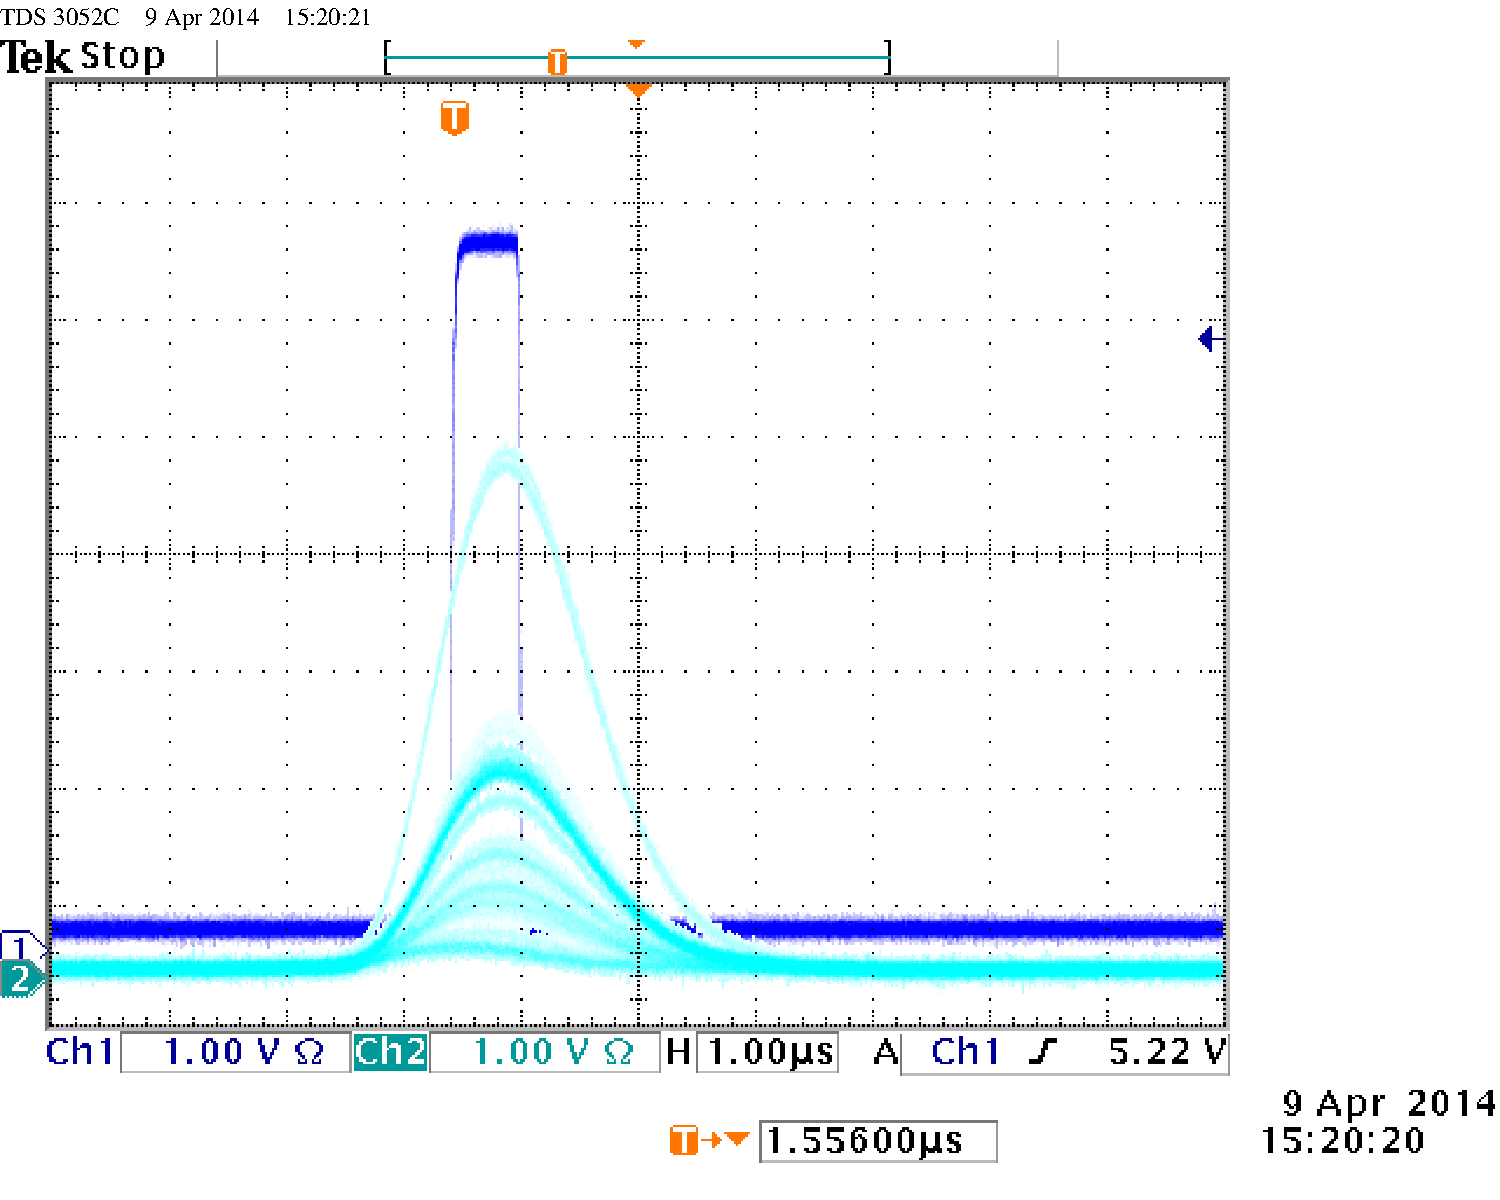
\includegraphics[width=.5\linewidth]{../Oszi-CFD.pdf}
    \caption{%
        Slow-Signal eines Photomultipliers zusammen mit dem
        Signal des Einkanalanalysators (SCA). Bild aus
        \parencite[Abbildung~2.8]{Ueding/525}. Ein Diskriminator ist zwar kein
        Einkanalanalysator, jedoch ist das Ausgangsbild vergleichbar.
    }
    \label{fig:oszi-cfd}
\end{figure}

Die Koinzidenzeinheit wird aus zwei digitalen Rechteckpulsen das Produkt
erstellen, also wieder einen Rechteckpulse, der nur in der überlappenden Region
1 ist. In Abbildung~\ref{fig:oszi-koinzidenz} ist das Oszillogramm von zwei
Eingängen gezeigt. Nach der Koinzidenz ist nur ein etwas schmalerer
Rechteckpuls zu sehen.

\begin{figure}[htbp]
    \centering
    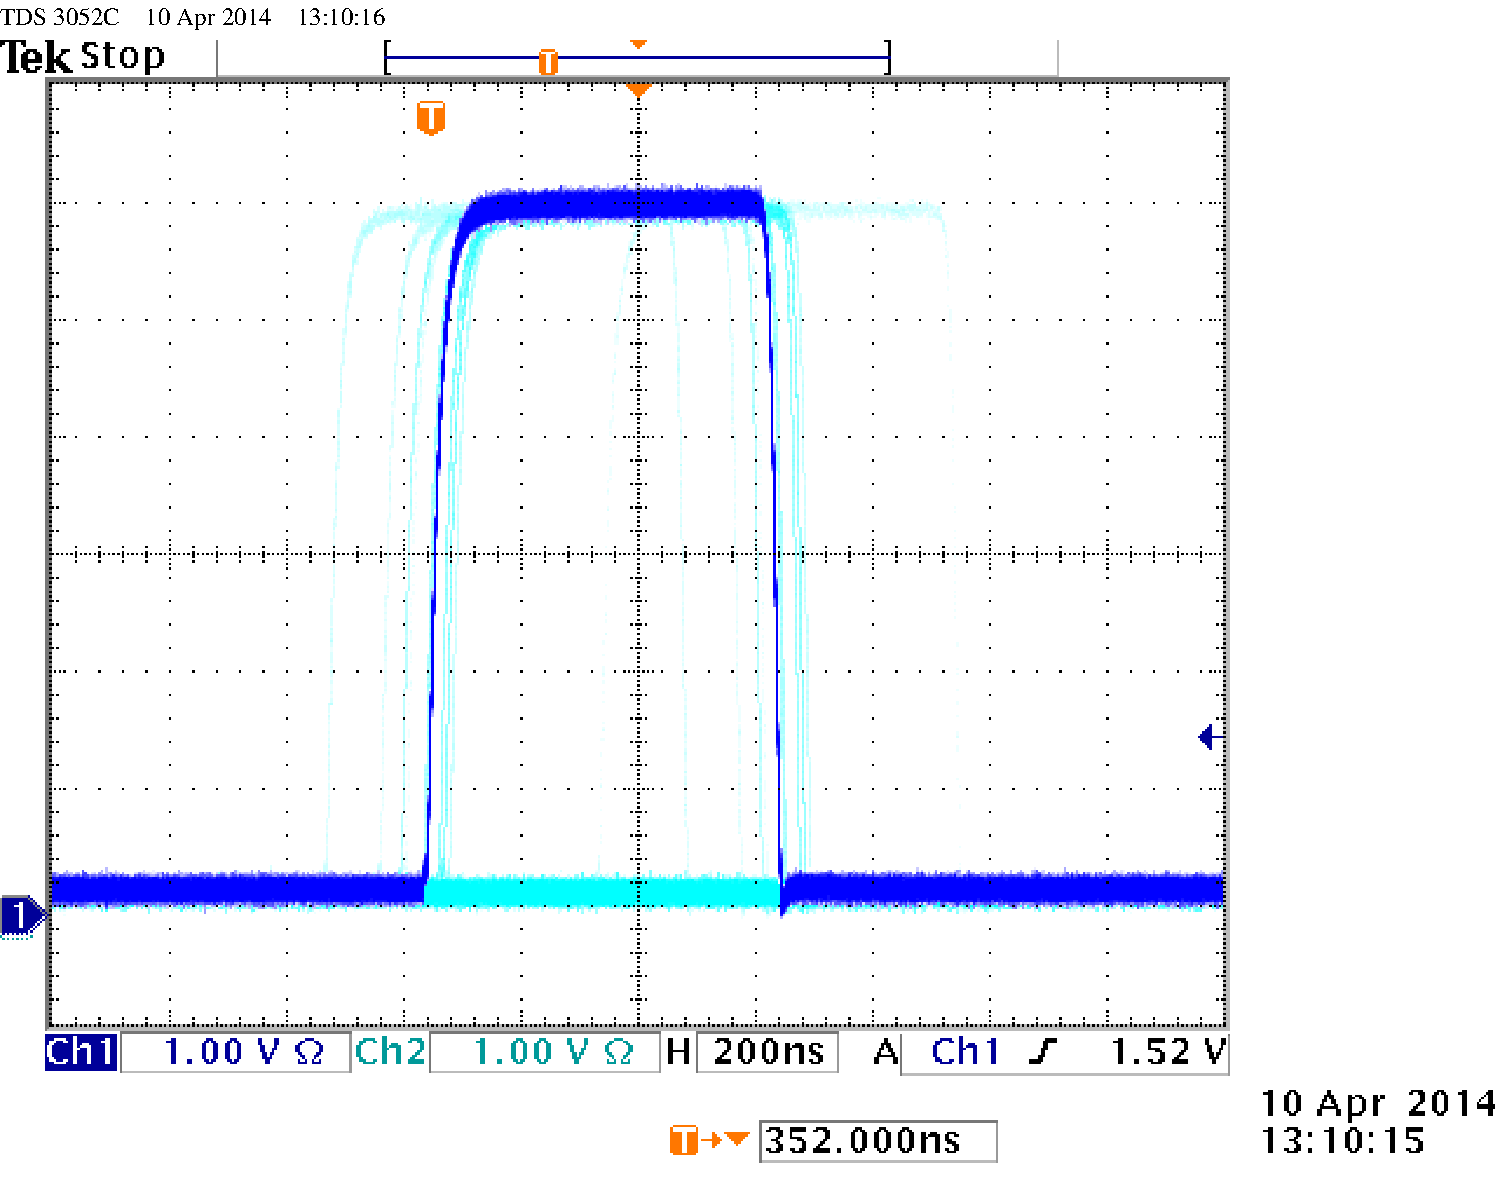
\includegraphics[width=.5\linewidth]{../Oszi-Koinzidenz.pdf}
    \caption{%
        Oszillogramm der Slow-Zweige von zwei verschiedenen Photomultiplier. Es
        wurde auf eins der Signale getriggert. Bild aus
        \parencite[Abbildung~2.24]{Ueding/525}.
    }
    \label{fig:oszi-koinzidenz}
\end{figure}

\subsection{Frage 3: Zufallskoinzidenzen}

Wir haben Gliederungspunkte eingefügt, damit wir besser auf die einzelnen
Fragen eingehen können.

\begin{quote}
    Die Zählrate für jeden einzelnen Zähler betrage etwa 1 Hz am
    Diskriminatorausgang.
    \begin{enumerate}
        \item
            \label{it:3-1-rate}
            Wie groß ist die theoretisch zu erwartende Rate der
            Zufallskoinzidenzen für eine der Dreifach-Koinzidenz-Schaltungen
            zur Messung der Winkelverteilung der Höhenstrahlung?

        \item
            \label{it:3-1-puls}
            Und für die Koinzidenz-Schaltung, die zur Messung des
            Pulshöhenspektrums verwendet wird?

        \item
            \label{it:3-1-tot}
            Wie groß sind jeweils die Totzeiten?

        \item
            \label{it:3-1-vorschlag}
            Machen Sie einen Vorschlag, wie die Rate der Zufallskoinzidenzen
            für eine der Dreifach-Koinzidenz-Schaltungen gemessen werden kann.
    \end{enumerate}
\end{quote}

\subsubsection{Teil \ref{it:3-1-rate}: Zufallskoinzidenzrate}

\newcommand\DtM{\Deltaup t_\text M}
\newcommand\DtO{\Deltaup t_\text O}
\newcommand\DtU{\Deltaup t_\text U}

Die Pulslängen der Diskriminatoren oben, unten und in der Mitte sind gegeben
mit:
\[
    \DtO = \SI{30}{\nano\second}
    \eqnsep
    \DtU = \SI{50}{\nano\second}
    \eqnsep
    \DtM = \SI{100}{\nano\second}.
\]

An jedem Zähler ist $f = \SI{1}{\hertz}$ als Durchschnitt angegeben. Wir nehmen
für unsere weiteren Überlegungen an, dass pro Intervall von \SI{1}{\second} ein
Impuls kommt, jedoch innerhalb des Intervalls zu einem beliebigen Zeitpunkt.
Wahrscheinlich sind die Pulse poissonverteilt, jedoch sind die Pulslängen so
kurz, dass eine Überlappung von zwei Impulsen das Endergebnis wahrscheinlich
nicht sonderlich verändern.

Innerhalb der Zeit $\DtM$ müssen auch die anderen Diskriminatoren ihr Signal
abgeben. Dies bedeutet also für die Koinzidenz von oberen und mittlerem
Detektor
\[
    - \DtO \leq t_\text O - t_\text M \leq \DtM,
\]
wobei $t_\text O$ und $t_\text M$ die Signalzeitpunkte innerhalb des Intervalls
sind. Sei $t_\text M$ beliebig. Somit muss $t_\text O$ ein Intervall der Breite
$\DtO + \DtM$ treffen, damit es eine Zweifachkoinzidenz gibt. Der Anteil
\[
    f \sbr{\DtO + \DtM}
\]
der Zeit steht also für Zweifachkoinzidenzen offen. Dazu muss jetzt das dritte
Signal ebenfalls so liegen, dass es die beiden vorherigen Überschneidet. Dies
ist immer gegeben, wenn $t_\text U$ innerhalb von $\DtO$ liegt, weil letzteres
das kürzeste Intervall ist. Im Prinzip kann es auch noch davor liegen, weil es
größer ist.

Da $\DtO < \DtM$, ist die Wahrscheinlichkeit, dass das kleinste komplett
innerhalb des größten ist, relativ groß und deckt das meiste damit ab. Somit
ist hier die Wahrscheinlichkeit, eine Koinzidenz zu erhalten:
\[
    f \sbr{\DtO + \DtU}.
\]

Die Rate ist somit:
\[
    f^3 \sbr{\DtO + \DtM} \sbr{\DtO + \DtU} \approx \SI{1.2e-14}{\hertz}.
\]

Da bei dieser Herleitung einige Überlappungsfälle nicht so genau behandelt
worden sind, haben wir dies noch mit Monte Carlo Methoden ausprobiert. Dieses
C++11 Programm zieht drei zufällige Zeiten innerhalb des Intervalls von einer
Sekunde. Dann prüft es, ob eine Dreifachkoinzidenz vorliegt.

\begin{Verbatim}[commandchars=\\\{\}]
\PY{c+c1}{// Copyright © 2014 Martin Ueding \PYZlt{}dev@martin\PYZhy{}ueding.de\PYZgt{}}
\PY{c+c1}{// Licensed under The GNU Public License Version 2 (or later)}

\PY{c+cp}{\PYZsh{}}\PY{c+cp}{include \PYZlt{}functional\PYZgt{}}
\PY{c+cp}{\PYZsh{}}\PY{c+cp}{include \PYZlt{}iostream\PYZgt{}}
\PY{c+cp}{\PYZsh{}}\PY{c+cp}{include \PYZlt{}random\PYZgt{}}

\PY{k+kt}{int} \PY{n+nf}{main}\PY{p}{(}\PY{p}{)} \PY{p}{\PYZob{}}
    \PY{k+kt}{double} \PY{n}{dtm}\PY{p}{\PYZob{}}\PY{l+m+mf}{100e\PYZhy{}5}\PY{p}{\PYZcb{}}\PY{p}{;}
    \PY{k+kt}{double} \PY{n}{dtu}\PY{p}{\PYZob{}}\PY{l+m+mf}{50e\PYZhy{}5}\PY{p}{\PYZcb{}}\PY{p}{;}
    \PY{k+kt}{double} \PY{n}{dto}\PY{p}{\PYZob{}}\PY{l+m+mf}{30e\PYZhy{}5}\PY{p}{\PYZcb{}}\PY{p}{;}

    \PY{k+kt}{unsigned} \PY{n}{iterations}\PY{p}{\PYZob{}}\PY{l+m+mi}{100000000}\PY{p}{\PYZcb{}}\PY{p}{;}
    \PY{k+kt}{unsigned} \PY{n}{triple}\PY{p}{\PYZob{}}\PY{l+m+mi}{0}\PY{p}{\PYZcb{}}\PY{p}{;}

    \PY{n}{std}\PY{o}{:}\PY{o}{:}\PY{n}{default\PYZus{}random\PYZus{}engine} \PY{n}{engine}\PY{p}{;}
    \PY{n}{std}\PY{o}{:}\PY{o}{:}\PY{n}{uniform\PYZus{}real\PYZus{}distribution}\PY{o}{\PYZlt{}}\PY{k+kt}{double}\PY{o}{\PYZgt{}} \PY{n}{distribution}\PY{p}{\PYZob{}}\PY{l+m+mf}{0.0}\PY{p}{,} \PY{l+m+mf}{1.0}\PY{p}{\PYZcb{}}\PY{p}{;}
    \PY{k}{auto} \PY{n}{die} \PY{o}{=} \PY{n}{std}\PY{o}{:}\PY{o}{:}\PY{n}{bind}\PY{p}{(}\PY{n}{distribution}\PY{p}{,} \PY{n}{engine}\PY{p}{)}\PY{p}{;}

    \PY{k}{for} \PY{p}{(}\PY{k+kt}{unsigned} \PY{n}{i}\PY{p}{\PYZob{}}\PY{l+m+mi}{0}\PY{p}{\PYZcb{}}\PY{p}{;} \PY{n}{i} \PY{o}{!}\PY{o}{=} \PY{n}{iterations}\PY{p}{;} \PY{o}{+}\PY{o}{+}\PY{n}{i}\PY{p}{)} \PY{p}{\PYZob{}}
        \PY{k+kt}{double} \PY{n}{tm}\PY{p}{\PYZob{}}\PY{n}{die}\PY{p}{(}\PY{p}{)}\PY{p}{\PYZcb{}}\PY{p}{;}
        \PY{k+kt}{double} \PY{n}{tu}\PY{p}{\PYZob{}}\PY{n}{die}\PY{p}{(}\PY{p}{)}\PY{p}{\PYZcb{}}\PY{p}{;}
        \PY{k+kt}{double} \PY{n}{to}\PY{p}{\PYZob{}}\PY{n}{die}\PY{p}{(}\PY{p}{)}\PY{p}{\PYZcb{}}\PY{p}{;}

        \PY{c+c1}{// Compute coincidence between M and U.}
        \PY{k+kt}{bool} \PY{n}{m\PYZus{}and\PYZus{}u}\PY{p}{\PYZob{}}\PY{o}{\PYZhy{}}\PY{n}{dtu} \PY{o}{\PYZlt{}}\PY{o}{=} \PY{n}{tu} \PY{o}{\PYZhy{}} \PY{n}{tm} \PY{o}{\PYZam{}}\PY{o}{\PYZam{}} \PY{n}{tu} \PY{o}{\PYZhy{}} \PY{n}{tm} \PY{o}{\PYZlt{}}\PY{o}{=} \PY{n}{dtm}\PY{p}{\PYZcb{}}\PY{p}{;}
        \PY{k}{if} \PY{p}{(}\PY{o}{!}\PY{n}{m\PYZus{}and\PYZus{}u}\PY{p}{)} \PY{p}{\PYZob{}} \PY{k}{continue}\PY{p}{;} \PY{p}{\PYZcb{}}

        \PY{k+kt}{bool} \PY{n}{m\PYZus{}and\PYZus{}o}\PY{p}{\PYZob{}}\PY{o}{\PYZhy{}}\PY{n}{dto} \PY{o}{\PYZlt{}}\PY{o}{=} \PY{n}{to} \PY{o}{\PYZhy{}} \PY{n}{tm} \PY{o}{\PYZam{}}\PY{o}{\PYZam{}} \PY{n}{to} \PY{o}{\PYZhy{}} \PY{n}{tm} \PY{o}{\PYZlt{}}\PY{o}{=} \PY{n}{dtm}\PY{p}{\PYZcb{}}\PY{p}{;}
        \PY{k}{if} \PY{p}{(}\PY{o}{!}\PY{n}{m\PYZus{}and\PYZus{}o}\PY{p}{)} \PY{p}{\PYZob{}} \PY{k}{continue}\PY{p}{;} \PY{p}{\PYZcb{}}

        \PY{k+kt}{bool} \PY{n}{u\PYZus{}and\PYZus{}o}\PY{p}{\PYZob{}}\PY{o}{\PYZhy{}}\PY{n}{dto} \PY{o}{\PYZlt{}}\PY{o}{=} \PY{n}{to} \PY{o}{\PYZhy{}} \PY{n}{tu} \PY{o}{\PYZam{}}\PY{o}{\PYZam{}} \PY{n}{to} \PY{o}{\PYZhy{}} \PY{n}{tu} \PY{o}{\PYZlt{}}\PY{o}{=} \PY{n}{dtu}\PY{p}{\PYZcb{}}\PY{p}{;}
        \PY{k}{if} \PY{p}{(}\PY{o}{!}\PY{n}{u\PYZus{}and\PYZus{}o}\PY{p}{)} \PY{p}{\PYZob{}} \PY{k}{continue}\PY{p}{;} \PY{p}{\PYZcb{}}

        \PY{c+c1}{// All three match up, this is a triple coincidence.}
        \PY{o}{+}\PY{o}{+}\PY{n}{triple}\PY{p}{;}
    \PY{p}{\PYZcb{}}

    \PY{n}{std}\PY{o}{:}\PY{o}{:}\PY{n}{cout} \PY{o}{\PYZlt{}}\PY{o}{\PYZlt{}} \PY{n}{triple} \PY{o}{\PYZlt{}}\PY{o}{\PYZlt{}} \PY{l+s}{\PYZdq{}}\PY{l+s}{ / }\PY{l+s}{\PYZdq{}} \PY{o}{\PYZlt{}}\PY{o}{\PYZlt{}} \PY{n}{iterations} \PY{o}{\PYZlt{}}\PY{o}{\PYZlt{}} \PY{l+s}{\PYZdq{}}\PY{l+s}{: }\PY{l+s}{\PYZdq{}}
        \PY{o}{\PYZlt{}}\PY{o}{\PYZlt{}} \PY{k}{static\PYZus{}cast}\PY{o}{\PYZlt{}}\PY{k+kt}{double}\PY{o}{\PYZgt{}}\PY{p}{(}\PY{n}{triple}\PY{p}{)} \PY{o}{/} \PY{n}{iterations} \PY{o}{\PYZlt{}}\PY{o}{\PYZlt{}} \PY{n}{std}\PY{o}{:}\PY{o}{:}\PY{n}{endl}\PY{p}{;}

    \PY{k}{return} \PY{l+m+mi}{0}\PY{p}{;}
\PY{p}{\PYZcb{}}
\end{Verbatim}


Die Daten aus der Anleitung erhält man mit \texttt{e-9}, also nano als Basis.
Wir haben mit \texttt{e-3} bis \texttt{e-5} laufen lassen, danach wurde die
Laufzeit zu lang. Verringert man die Größenordnung der Diskriminatorsignale um
eins, so verringert sich die Größenordnung der Zufallskoinzidenzrate um zwei.
Daher extrapolieren wir dies auf eine erwartete Rate von \SI{9e-15}{\hertz}.
Dies deckt sich gut mit den vorherigen Überlegungen.

\subsubsection{Teil \ref{it:3-1-puls}: Für Pulshöhenspektrum}

Für das Pulshöhenspektrum wird folgende Koinzidenz aufgebaut:
\[
    [\mathrm D23 \lor \mathrm D24 \lor \mathrm D1 \lor \mathrm D2] \land
    \mathrm D12.
\]

Daher muss jetzt in nur einem der oberen Detektoren ein Ereignis gleichzeitig
mit dem unteren Detektor stattfinden, damit es eine Zufallskoinzidenz gibt. Wir
nehmen an, dass die Zufallsereignisse in den oberen vier Detektoren nicht
gleichzeitig auftreten. Dies führt dazu, dass die Gesamtrate das vierfache der
einfachen Koinzidenzrate ist:
\[
    4 f^2 \sbr{\DtO + \DtU} \approx \SI{3.2e-7}{\hertz}.
\]
Auch diese Rate ist wieder sehr klein.

\subsubsection{Teil \ref{it:3-1-tot}: Totzeiten}

Die Totzeiten sind die Zeiten, in denen ein zweites legitimes Ereignis nicht
aufgelöst werden kann. Diese Zeit ist ein klein wenig größer als die Länge des
kürzesten Diskriminatorsignals. Angenommen, alle Diskriminatoren lösen
gleichzeitig aus. Die Koinzidenz besteht solange, wie alle Diskriminatoren ein
Signal senden. Danach verschwindet die Koinzidenz und der Diskriminator mit der
kürzesten Signaldauer kann wieder von einem legitimen Ereignis ausgelöst
werden. In beiden Fällen ist dies $\DtO = \SI{30}{\nano\second}$.

\subsubsection{Teil \ref{it:3-1-vorschlag}: Vorschlag zur Messung}

Zufällige Ereignisse sind miteinander überhaupt nicht korreliert. Daher kann
man die Diskriminatorsignale beliebig verzögern und erhält die gleiche
Zufallskoinzidenzrate. Die legitimen Signale verschwinden jedoch bei zu großen
Verzögerungen.

Baut man also eine zweite Koinzidenzschaltungen auf, in der die Signale stark
verzögert ankommen auf, gibt diese die Zufallskoinzidenzrate. Ein Teilchen kann
die Detektoren gar nicht derart durchlaufen, dass es mit großen Verzögerungen
ein Signal gibt.

\subsection{Frage 4: Bethe-Bloch und Landau}

\begin{quote}
    Welchen inhaltlichen Zusammenhang haben Bethe-Bloch-Gleichung und
    Landau-Verteilung?
\end{quote}

In den Abschnitten §\ref{sec:bethe-bloch} und §\ref{sec:landauverteilung} haben
wir etwas zur Bethe-Bloch-Gleichung und der Landauverteilung geschrieben. Die
Bethe-Bloch-Gleichung gibt den mittleren Energieverlust an, die
Landauverteilung die tatsächliche Verteilung der Energieverluste an. Der
Mittelwert der Landauverteilung ist entsprechend der Wert, den die
Bethe-Bloch-Gleichung gibt.

\subsection{Frage 5: Pulshöhenspektrum}

\begin{quote}
    \begin{enumerate}
        \item
            \label{it:1-5-beitrag}
            Welche Beiträge hat das Pulshöhenspektrum?

        \item
            \label{it:1-5-einfluss}
            Welche physikalischen und apparativen Einflüsse bestimmen die Form
            des Pulshöhenspektrums?

        \item
            \label{it:1-5-unterschied}
            Wie unterscheiden sich zwei Pulshöhenspektren, wenn diese mit und
            ohne aktiven Gate-Eingang aufgenommen werden?
    \end{enumerate}
\end{quote}

\subsubsection{Teil \ref{it:1-5-beitrag}: Beiträge}

Der Großteil des Spektrums orientiert sich stark am Pionenspektrum in der
Atmosphäre. Dieses sieht dem Protonenspektrum ebenfalls ähnlich. Die Abweichungen ergeben sich bei kleinen Energien durch den
Zerfall der Myonen. Bei großen Energien erzeugen die Pionen weitere Pionen, die
dann jedoch nur weniger energetische Myonen erzeugen. Daher gibt es weniger
hochenergetische Myonen. \parencite[§6.1, §7.2]{Grupen/Astroteilchenphysik}

Ebenfalls können die Myonen noch durch andere Teilchen als die Pionen
entstehen, \parencite[115]{Grupen/Astroteilchenphysik} nennt charmante Mesonen
als weitere Quelle. Weiter werden Elektronen und Photonen als Beiträge genannt,
die den Detektor auslösen können.

\subsubsection{Teil \ref{it:1-5-einfluss}: Einflüsse}

Die obere und untere Grenze in der Energie des MCA schneiden das Spektrum
entsprechend ab. Hängt die Ansprechwahrscheinlichkeit des Detektors von der
Energie ab, so verzerrt dies das Spektrum. Andere Nichtlinearitäten verzerren
das Spektrum ebenso.

% TODO Antwort einfügen.

\subsubsection{Teil \ref{it:1-5-unterschied}: Unterschiede}

Schließt man an das Gate nichts an, werden gar keine Ereignisse aufgenommen.
Ist es immer offen, wird der Untergrund nicht mehr herausgefiltert. Man hat
also auf der Niederenergetischen Flanke mehr Ereignisse als mit aktivem Gate.
Außerdem können die Teilchen dann aus jeder Richtung kommen, es handelt sich
nicht mehr um Teilchen, deren Flugbahn nahe der Senkrechten liegt.

\subsection{Frage 6: Pulshöhenspektrum und Schwellenkurve}

\begin{quote}
    Wie hängen Pulshöhenspektrum und Schwellenkurve zusammen? Wie ändert sich
    die Form der Schwellenkurve, wenn man die Anzahl der Koinzidenzsignale
    anstelle der Diskriminatorsignale betrachtet?
\end{quote}

Im Pulshöhenspektrum sind die Zählraten für verschiedene Energien dargestellt.
Die Schwellenkurve gibt die Zählrate gegen die Diskriminatorschwelle, welche
die untere Grenze der Energie ist. Ist das Pulshöhenspektrum als $n(E)$
gegeben, so ist die Schwellenkurve $S(E)$
\[
    S(E) = \int_E^\infty \dif E' \, n(E'),
\]
also die Anzahl aller Ereignisse mit einer Energie oberhalb der Schwelle.

\subsection{Frage 7: LabVIEW Programm}

\begin{quote}
    Welche Funktion erfüllt das in Abbildung 5 gezeigte LabVIEW-Programm?
\end{quote}

Wir haben das Programm mit einigen Anmerkungen versehen, siehe
Abbildung~\ref{fig:labview-test}.

\begin{figure}[htbp]
    \centering
    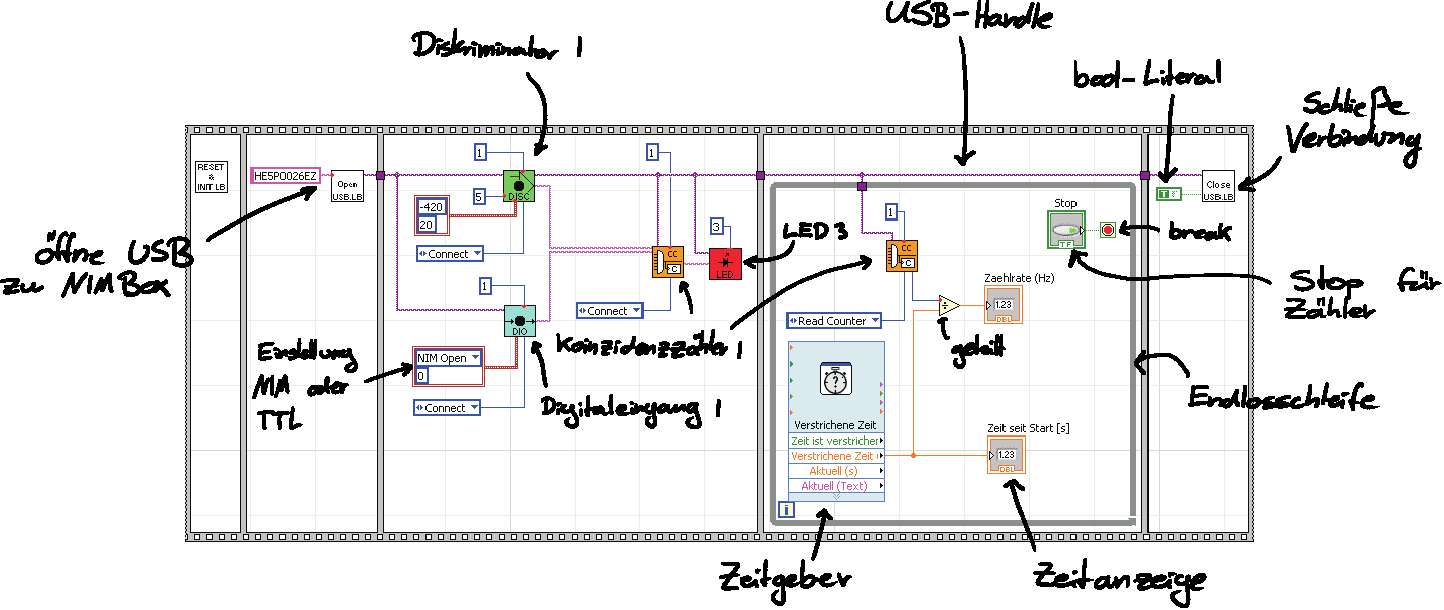
\includegraphics[width=\linewidth]{../Programm-crop.pdf}
    \caption{%
        LabVIEW Programm aus \parencite[Abbildung~5]{physik512-Anleitung}.
    }
    \label{fig:labview-test}
\end{figure}

Dieses Programm realisiert eine Zählratenbestimmung mit einem Zähler mit
Diskriminator und Gate. Die Bauteile im Detail:

\subsubsection{Erstes Bild: Reset}

Im ersten Bild des Filmstreifens wird die NIMBox zurückgesetzt und
initialisiert.

\subsubsection{Zweites Bild: Init}

Hier wird die Verbindung zur NIMBox aufgebaut und die USB Verbindung als handle
(dunkelviolett) zum nächsten Bild gegeben. Mit diesem handle können alle Module
auf die richtige NIMBox bezogen werden.

\subsubsection{Drittes Bild: Setup}

Oben ist das violette handle für die USB-Verbindung zum nächsten Bild
geschleift. Dieses handle ist ebenfalls an alle Bauteile angeschlossen.

Das grüne ist ein Diskriminator. Dieser bekommt von oben eine 1, so dass dies
der erste Diskriminator in der Box ist. Die drei weiteren Eingänge, $-420$, 20
und 5 stehen für die Schwelle, Hystere in \si{\milli\volt} bzw. für die Dauer
des Ausgangspulses in \SI{10}{\nano\second}. Das „Connect“ führt hier dazu,
dass dieser Diskriminator so konfiguriert wird.

Das türkise Element ist für digitale Ein- und Ausgabe (digitale IO). Auch
dieses ist das erste in der Box. Mit einem „Connect“ wird es ebenfalls
angeschlossen. Der Cluster mit Parametern gibt noch an, dass NIM anstelle von
TTL als Übertragunsstandard gewählt worden ist. Dies muss mit der Position des
physischen Jumpers übereinstimmen. Dieses Modul wird dazu benutzt, digitale
Signale in das Programm zu bekommen.

Die Signale von Diskriminator und digitaler Eingabe werden zusammen auf einen
Koinzidenzzähler (orange) gelegt. Dies ist der erste in der Box und wird auch
so angeschlossen.

Dessen Ausgang geht wiederum auf eine LED, diesmal die dritte in der Box.

\subsubsection{Viertes Bild: Schleife}

Auch im vierten Bild kommt das handle für die USB-Verbindung an und wird
weitergegeben. Das handle wird in die Endlosschleife hineingegeben. Dort wird
der erste Koinzidenzzähler (dunkles orange) ausgelesen und durch die bis
dorthin verstrichene Zeit geteilt. Diese Zeit liefert ein Zeitgeber (hellblau).
In der Ausgabe erscheint die Rate sowie die Zeit seit Start. Um die Schleife
verlassen zu können ist ein Schalter als Abbruchbedingung in die Vorderansicht
eingebaut.

\subsubsection{Fünftes Bild: Ende}

Zuletzt wird die USB-Verbindung getrennt. Da die boolsche Konstante auf wahr
gesetzt ist, wird das Programm im Speicher der NIMBox gespeichert.

\section{Vorbereitungsfragen zur Myonenlebensdauer}

Dies sind die Vorbereitungsfragen aus \parencite[14]{physik512-Anleitung}.

\subsection{Frage 1: Myonen und Antimyonen}

\begin{quote}
    Es kommen sowohl Myonen als auch Antimyonen auf der Erdoberfläche an.
    Welcher atomphysikalische Prozeß ist für Myonen möglich, aber nicht für
    Antimyonen? Wie beeinflußt das qualitativ die in diesem Versuch gemessene
    Lebensdauer?
\end{quote}

Der Zerfall des Myons verläuft wie folgt \parencite[144]{Povh/Teilchen_Kerne}:
\[
    \muup^- \to \nuup_\muup + \bar \nuup_\eup + \eup^-
    \eqnsep
    \muup^+ \to \bar \nuup_\muup + \nuup_\eup + \eup^+.
\]

Die Gleichheit der Lebensdauern ist auf \num{e-4} überprüft worden
\parencite{Wikipedia/Muon}. Dies bezieht sich aber nur die Myonen alleine im
Vakuum, siehe weiter unten.

Neutrinos treten nur mit negativer Helizität auf, sind also linkshändig.
Antineutrinos haben dagegen immer positive Helizität. Betrachtet man die
Zerfälle, in denen das Elektron/Positron maximalen Impuls übernimmt, so bewegen
sich beide Neutrinos in die entgegengesetzte Richtung. Deren Gesamtspin ist 0,
aufgrund der entgegengesetzten Helizitäten. Somit muss das Elektron/Position
den gleichen Spin tragen wie das Myon/Antimyon. Positronen, die durch schwache
Wechselwirkung zerfallen sind fast immer rechtshändig, also mit positiver
Helizität. Dies bedeutet, dass sich das Positron fast immer in den Halbraum, in
den der Spin des Antimyons zeigt, bewegt.
\parencite[§3]{Egede/Parity_Violation}

Die meisten Antimyonen, die auf der Erdoberfläche ankommen, sind linkshändig.
Dies liegt daran, dass sie durch den Zerfall des $\piup^+$-Mesons erzeugt
werden. Das entstehende Neutrino ist immer linkshändig. Im Ruhesystem des Pions
ist das Myon ebenfalls Linkshändig, da der Spin des Pions null ist. Jedoch
bewegt sich das Pion schnell auf die Erde zu. Wurde das Myon vom Pion in
Richtung Erde ausgesandt, so ist es linkshändig und schnell. Wurde es in die
andere Richtung ausgesandt, ist es rechtshändig und langsamer. Von den
langsamen Myonen zerfallen mehr, so dass auf der Erdoberfläche die
linkshändigen ankommen, deren Spin Richtung Zenit zeigt.
\parencite[S.~29f]{Egede/Parity_Violation}

Dies erklärt eine Paritätsverletzung, jedoch keinen Unterschied in der
Lebensdauer. Allerdings gelten die vorherigen Betrachtungen auch nur für das
Vakuum.

In Material, das aus Materie (also nicht aus Antimaterie) besteht, können die
Myonen an Atomkerne binden und einen elektronischen Zustand einnehmen. Dadurch
verlieren die Myonen ihren Spin, die Paritätsverletzung betrifft Antimyonen
daher deutlich stärker. \parencite[30]{Egede/Parity_Violation}

Der Fluß der Myonen wird durch den Einfang durch Atomkerne in der Luft
ebenfalls reduziert. \parencite{TwoBs/Myon_Decay}

Außerdem kann ein Myon zusammen mit einem Proton ein Neutron erzeugen. Dadurch
verkürzt sich die Lebenszeit des Myons im Vergleich zum Antimyon.
\parencite{Rennie/Myon_Decay}

Daher ist zu erwarten, dass wir nicht einen exponentiellen Abfall sehen,
sondern eine Überlagerung von zwei exponentiellen Zerfallskurven.

\subsection{Frage 2: Start und Stop}

\begin{quote}
    Machen Sie einen Vorschlag, wie man unter Verwendung von Diskriminatoren,
    Verzögerungskabeln und Koinzidenz-Schaltungen die \textsc{Start}-und
    \textsc{Stop}-Impulse erzeugen kann.
\end{quote}

Ähnlich wie bei der Lebensdauermessung des metastabilen Zustands in Versuch~525
lassen wir den ersten Detektor das \textsc{Start}-Signal liefern. Der
Diskriminator muss entsprechend eingestellt werden, dass nur Ereignisse
registriert werden, die von einem Myon stammen. Um zufällige Ereignisse besser
herausfiltern zu können, müssen oberer und unterer Detektor gleichzeitig ein
Signal liefern, damit dies als \textsc{Start}-Signal zählt. Der
\textsc{Stop}-Impuls kommt alleine vom zweiten Detektor, in dem das Myon zur
Ruhe gekommen ist.

Da in der Anleitung nur Diskriminatoren und keine Einkanalanalysatoren erwähnt
werden, benutzen wir wahrscheinlich keine Fast-Slow-Koinzidenzschaltung,
sondern benutzten nur den Fast-Zweig aus dieser.

Da es theoretisch möglich ist, dass das Myon sofort zerfällt, sollte das
\textsc{Stop}-Signal etwas verzögert werden, damit das \textsc{Stop}-Signal
nach dem \textsc{Start}-Signal kommt. Die Lebensdauer bestimmt sich aus dem
exponentiellen Abfall, so dass eine derartige Verschiebung nichts ändert.

\subsection{Frage 3: Blockschaltbild}

\begin{quote}
    Entwerfen Sie das Blockschaltbild für Messkreis und Monitorkreis.
\end{quote}

Siehe Abbildung~\ref{fig:aufbau-muon}.

\subsection{Frage 4: Zeitintervalle}

\begin{quote}
    Können Sie eine andere Gestaltung der Zeitintervalle vorschlagen, die die
    Genauigkeit der Myonlebensdauerbestimmung optimieren würde?
\end{quote}

Die Intervalleinteilung in der Anleitung ist linear. Da ein exponentieller
Abfall in der Kurve zu erwarten ist, werden in den ersten Intervallen mehr
Ereignisse gemessen als in den letzten. Dadurch ist der relative Fehler in den
ersten Intervallen kleiner. Verkleinert man die ersten und streckt dafür die
letzten Intervalle exponentiell, kann man dadurch den relativen Fehler in allen
Intervallen gleich bekommen.

\subsection{Frage 5: Verzögerung}

\begin{quote}
    Das aus der Apparatur kommende \textsc{Start}-Signal wird gegenüber dem
    \textsc{Stop}-Signal um ca. \SI{100}{\nano\second} verzögert. Warum ist das
    notwendig? Wie wirkt es sich auf das Messergebnis aus?
\end{quote}

So, wie es in Abbildung~\ref{fig:aufbau-muon} gezeigt ist, würde ein Teilchen,
das gleichzeitig ein Ereignis in Detektor~1 und 2 auslöst, sowohl ein
\textsc{Start}- als auch ein \textsc{Stop}-Signal senden. Durch die Verzögerung
des \textsc{Start}-Signals wird dafür gesorgt, dass das ungewünschte
\textsc{Stop}-Signal keine Wirkung hat.

Das Messergebnis wird dadurch nur zu kleineren Zeiten verschoben, Die
Lebenszeit $\tau$ der Myonen erhalten wir jedoch aus dem exponentiellen Abfall
der Zählrate. Diese Verschiebung ändert daran nichts.

\subsection{Frage 6: Scheinbare Myonzerfälle}

\begin{quote}
    Wie können scheinbare Myonzerfälle zustandekommen? Welche Messgrößen
    braucht man, um die erwartete Anzahl von Zufallsereignissen berechnen zu
    können?
\end{quote}

Kommt es innerhalb der Messzeit in den \textsc{Stop}-Detektor zu
Zufallsereignissen, werden diese als ein Ereignis mit entsprechend kürzerer
Lebensdauer registriert. Der Zerfall des Myons erfolgt dann außerhalb des
Messzeitraums. Um die Rate berechnen zu können brauchen wir die Rate der
Koinzidenzen, also der Teilchen, die Detektor 1 durchqueren und in Detektor 2
ebenfalls ein Signal auslösen, $f_{1,2}$. Dann benötigen wir die Lebensdauer
des Myons, $\tau$. Außerdem brauchen wir die Rate aller Ereignisse, die in
Detektor 2 Signale auslösen, $f$ (zum Beispiel kosmische Gammastrahlung).

Ein zufälliger Impuls muss den Messzeitraum, der $\tau$ lang ist, treffen.
Diese treten mit der Rate $f_{1,2}$ auf, so dass die Wahrscheinlichkeit, ein
Zufallsereignis zu erzeugen, $f_{1,2} \tau$ ist. Die Rate der Zufallsereignisse
ist damit dann $f_{1,2} f \tau$.

Wenn die Frequenzen im Bereich von \SI{1}{\hertz} sind, so ist die Rate der
Zufallsereignisse im Bereich \SI{e-5}{\hertz}, da die erwartete Lebensdauer im
Bereich \SI{e-6}{\micro\second} liegt.

% TODO Antwort einfügen.

\chapter{Winkelverteilung}

Um die Übersicht über die vielen kleinen Schritte zu gewährleisten, möchten wir
hier erst einmal die Schritte grob zusammenstellen:

\begin{enumerate}
    \item
        Einstellung der Diskriminatorschwellen um den Untergrund zu filtern.
        Die zugehörige Messung läuft über Nacht. Siehe
        §\ref{sec:einstellung_diskriminatorschwelle}.

    \item
        Finden der optimalen Verzögerung der Signale, die in den MCA gehen,
        damit deren Überschneidung maximiert wird. Siehe
        §\ref{sec:optimieren_verzoegerung}.

    \item
        Aufnahme der Winkelverteilung, also Zählrate über alle Energien gegen
        Winkel. Diese Messung läuft über Wochen. Siehe
        §\ref{sec:langzeit_winkel}.

    \item
        Aufnahme eines Pulshöhenspektrums der Höhenstrahlung, also letztlich
        Zählrate gegen Energie. Dies läuft ebenfalls über Wochen. Siehe
        §\ref{sec:langzeit_puls}.
\end{enumerate}

\section{Aufbau, Geräte}

\subsection{Zählerring}

Das Detektorsystem besteht aus 24 ringförmig angeordneten
Szintillationszählern, die um einen zentralen Zähler angeordnet sind, siehe
Abbildung~\ref{fig:detektoren}. Der ganze Ring steht senkrecht, so dass die
Winkelverteilung im Bezug auf den Zenit bestimmt werden kann.

\begin{figure}[htbp]
    \centering
    \tikzsetnextfilename{detektoren}
    \begin{tikzpicture}
        \draw[->] (45:7) -- ++(0, 1) node[above, midway, sloped] {Zenit};

        %< for i in range(1, 25): >%
        \node[draw, rectangle, rotate=<< - i * 15 >>, label=90:Z<< i >>]
        (Z<< i >>) at (<< 90 - i * 15 >>:5) {\phantom{----}};
        %< endfor >%

        \node[draw, circle] (Z25) at (0, 0) {Z25};

    \end{tikzpicture}
    \caption{%
        Anordnung der Detektoren.
    }
    \label{fig:detektoren}
\end{figure}

\subsection{Elektronik}

\subsubsection{Diskriminatoren}

An jeden Detektor ist ein Diskriminator angeschlossen. Damit werden die
analogen Pulse in digitale Pulse umgewandelt.

\subsubsection{Verteiler}

Der mittlere Zähler Z25 wird für die Koinzidenz von allen Detektorpaaren
benötigt. Daher wird dessen Signal nach dem Diskriminator durch einen Fanout
zwölffach aufgefächert.

\subsubsection{Koinzidenz}

Ziel der Koinzidenz ist, nur solche Ereignisse zu filtern, bei denen ein
Teilchen genau durch die Mitte und ein gegenüberliegendes Detektorpaar
fliegt. Um dies zu filtern, gehen die digitalen Signale von zwei
gegenüberliegenden Detektoren sowie des mittleren Detektors in eine
Koinzidenzeinheit. Dies ist für zwei Detektorpaare in
Abbildung~\ref{fig:koinzidenz} dargestellt.

\begin{figure}[htbp]
    \centering
    \tikzsetnextfilename{koinzidenz}
    \begin{tikzpicture}

        %< for i in range(1, 25): >%
        \node[draw, circle] (Z<< i >>) at (<< 90 - i * 15 >>:7) {Z<< i >>};
        \node[draw, rectangle] (D<< i >>) at (<< 90 - i * 15 >>:5) {D<< i >>};
        \draw[->] (Z<< i >>) -- (D<< i >>);
        %< endfor >%

        \node[draw, circle] (Z25) at (0, 0) {Z25};

        \node[draw, rectangle] (D25) [below=of Z25] {D25};

        \node[draw, rectangle] (fan) [below=of D25] {Fanout};

        \node[draw, rectangle] (con1) [right=of Z25] {Koinzidenz};
        \node[draw, rectangle] (con2) [left=of Z25] {Koinzidenz};

        \begin{scope}[->]
            \draw (Z25) -- (D25);
        \end{scope}

        \begin{scope}[->, dashed]
            \draw (D25) -- (fan);

            \draw (fan) -- (con1);
            \draw (fan) -- (con2);

            \draw (D2) -- (con2);
            \draw (D14) -- (con2);

            \draw (D22) -- (con1);
            \draw (D10) -- (con1);
        \end{scope}

        \draw[->] (45:8) -- ++(0, 1) node[right, midway] {$\theta = 0$};

    \end{tikzpicture}
    \caption{%
        Anordnung der Detektoren. Zur Übersicht sind nur zwei
        Koinzidenzschaltungen eingezeichnet. Durchgezogene und gestrichelte
        Linien stehen für analoge bzw. digitale Signalübertragungen. Detektoren
        sind durch Kreise, Elektronik durch Rechtecke gekennzeichnet.
    }
    \label{fig:koinzidenz}
\end{figure}

\subsubsection{Zähler}

Zum einen benutzen wir die Zähler, die in der NIMBox eingebaut sind. Deren
Zählstand lässt sich am PC in LabVIEW ablesen. Zum anderen haben wir 10
Sichtzähler zur Verfügung, die wir für die Messung der Zufallskoinzidenzrate
benutzen werden.

\section{Justierung}

\subsection{Einstellung der Diskriminatorschwelle}
\label{sec:einstellung_diskriminatorschwelle}

\subsubsection{Entwicklung der Schaltung}

Zur Ermittlung der optimalen Diskriminatorschwelle müssen wir eine
Schwellenkurve aufnehmen. Dies ist eine Kurve mit Zählrate gegen
Diskriminatorschwelle. Da wir von einer recht monoenergetischen Myonenstrahlung
ausgehen, erwarten wir eine Stufenfunktion mit einer Stufe. Bei kleinen
Schwellen werden wir den kompletten Untergrund mitnehmen. Ab der Schwelle, die
der Myonenstrahlung entspricht, erwarten wir einen Einbruch. Die
Diskriminatorschwelle wählen wir anschließend so, dass wir den Untergrund
filtern können, jedoch möglichst wenig von den Myonen verlieren.

Dazu konstruieren wir in LabVIEW eine Schaltung, die über Nacht die
verschiedenen Schwellen durchfährt und die Zählraten misst. Dabei müssen
folgende Daten für die weitere Durchführung aufgezeichet werden.

\begin{itemize}
    \item
        Gewählte Schwelle für Z12

    \item
        Anzahl Ereignisse in D12

    \item
        Anzahl der oder-Ereignisse

    \item
        Anzahl der Ereignisse in Z25

    \item
        Messdauer

    \item
        Anzahl der Koinzidenzen
\end{itemize}

Im Vorfeld haben wir uns überlegt, wie diese Programme grob aussehen müssten.
In Abbildung~\ref{fig:entwurf-1} ist der Teil, der die Koinzidenz
implementiert, gezeigt. Dort werden die Signale aus den Diskriminatoren über
drei oder-Gatter zusammengeführt. Zusammen mit dem Signal aus D12 gehen diese
dann in den Koinzidenzzähler. Dessen Logikausgang geben wir zur Kontrolle auf
eine LED sowie durch die Lemo-Buchse nach draußen.

\begin{figure}[htbp]
    \centering
    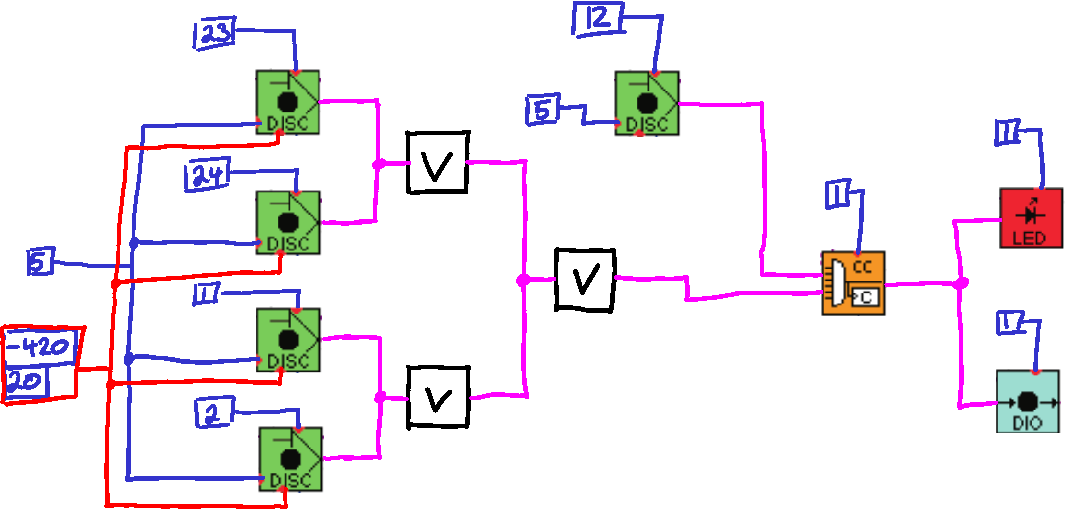
\includegraphics[width=\linewidth]{../Drawing-0001.pdf}
    \caption{%
        Entwurf einer LabVIEW Schaltung für die Koinzidenz.
    }
    \label{fig:entwurf-1}
\end{figure}

Um nun die verschiedenen Schwellen durchzumessen, müssen wir eine Schleife
konstruieren und die verschiedenen Schwellen eine gewisse Zeit lang messen.
Dazu halten wir eine \texttt{for}-Schleife für sinnvoll. Aus dem Index
errechnen wir die Schwelle und sammeln alle interessanten Daten in Arrays. Mit
Abbildung~\ref{fig:entwurf-2} haben wir unsere Skizze eingefügt.

Die Schwellenzahl, die Messdauer und der Schwellenschritt müssen noch
eingetragen werden. Dabei müssen wir darauf achten, dass die Messzeit bis zum
nächsten Morgen nicht überschritten wird.

In jedem Schleifendurchlauf wird die Schwelle berechnet und der Diskriminator
entsprechend eingestellt. Die Messzeit wird gewartet, bis entsprechend viele
Ereignisse im Koinzidenzzähler angekommen sind. Mit weiteren Zählern zählen wir
noch weitere Größen, die interessant werden können. Diese Werte geben wir durch
den „loop tunnel” in Arrays weiter.

\begin{figure}[htbp]
    \centering
    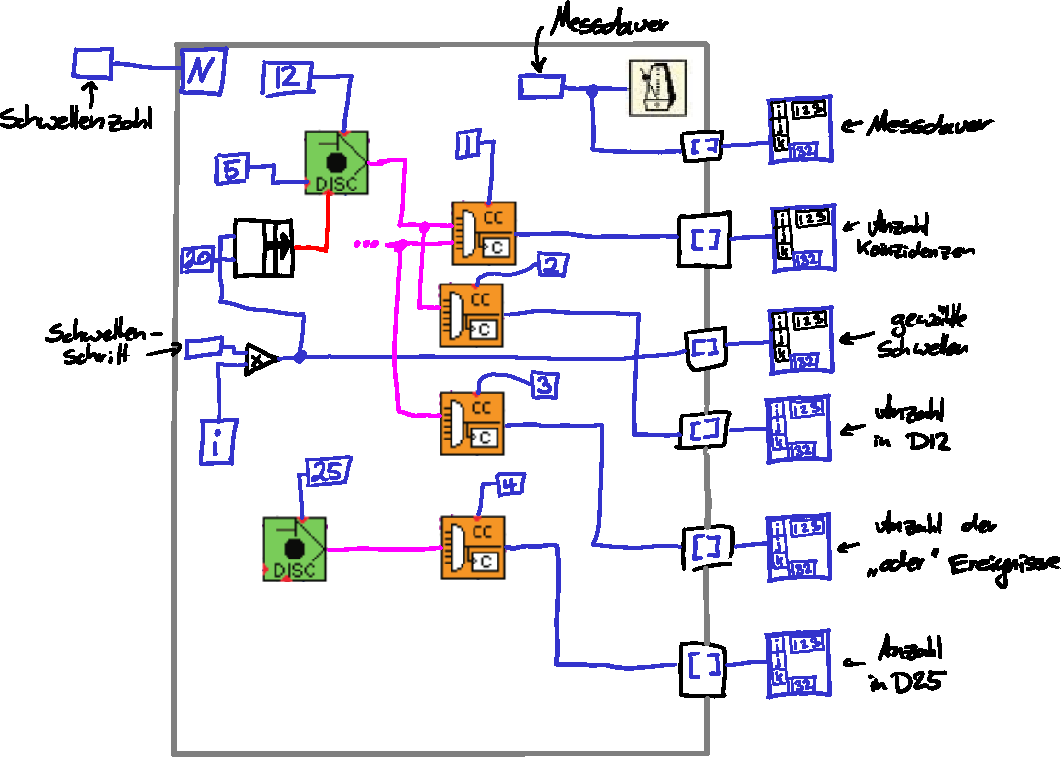
\includegraphics[width=\linewidth]{../Drawing-0002.pdf}
    \caption{%
        Entwurf einer LabVIEW Schaltung für das Durchmessen der Schwellen.
    }
    \label{fig:entwurf-2}
\end{figure}

Zuletzt speichern wir die Daten aus den Arrays ab. Dazu bündeln wir sie in ein
zweidimensionales Array und speichern es als Textdatei ab. Dies ist in
Abbildung~\ref{fig:entwurf-3} dargestellt.

\begin{figure}[htbp]
    \centering
    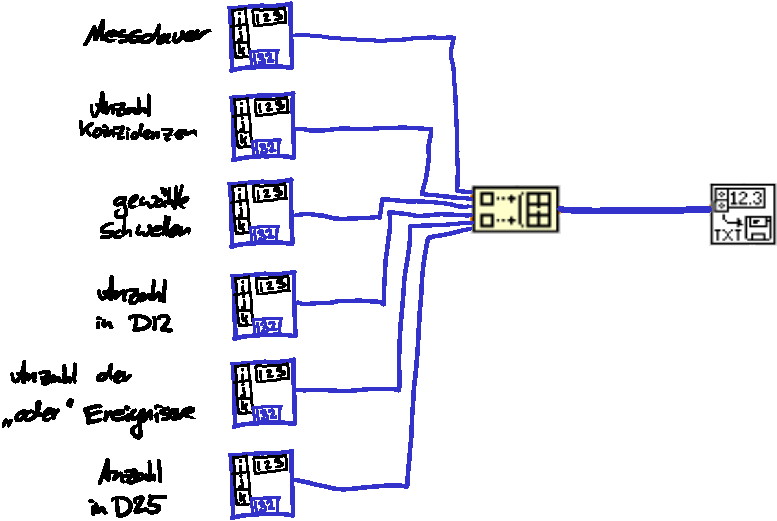
\includegraphics[width=.8\linewidth]{../Drawing-0003.pdf}
    \caption{%
        Entwurf einer LabVIEW Schaltung für das Speichern der Daten.
    }
    \label{fig:entwurf-3}
\end{figure}

Das endgültige Programm, das wir am ersten Versuchstag entwickelt haben, ist in
Abbildung~\ref{fig:labview-programm} gezeigt. Wir haben noch das Zurücksetzen
der Zähler eingefügt. Die Schwellen für die anderen Diskriminatoren haben wir
aus dem Programm kopiert, das für die Langzeitmessung benutzt wird.

\begin{landscape}
    \begin{figure}[htbp]
        \centering
        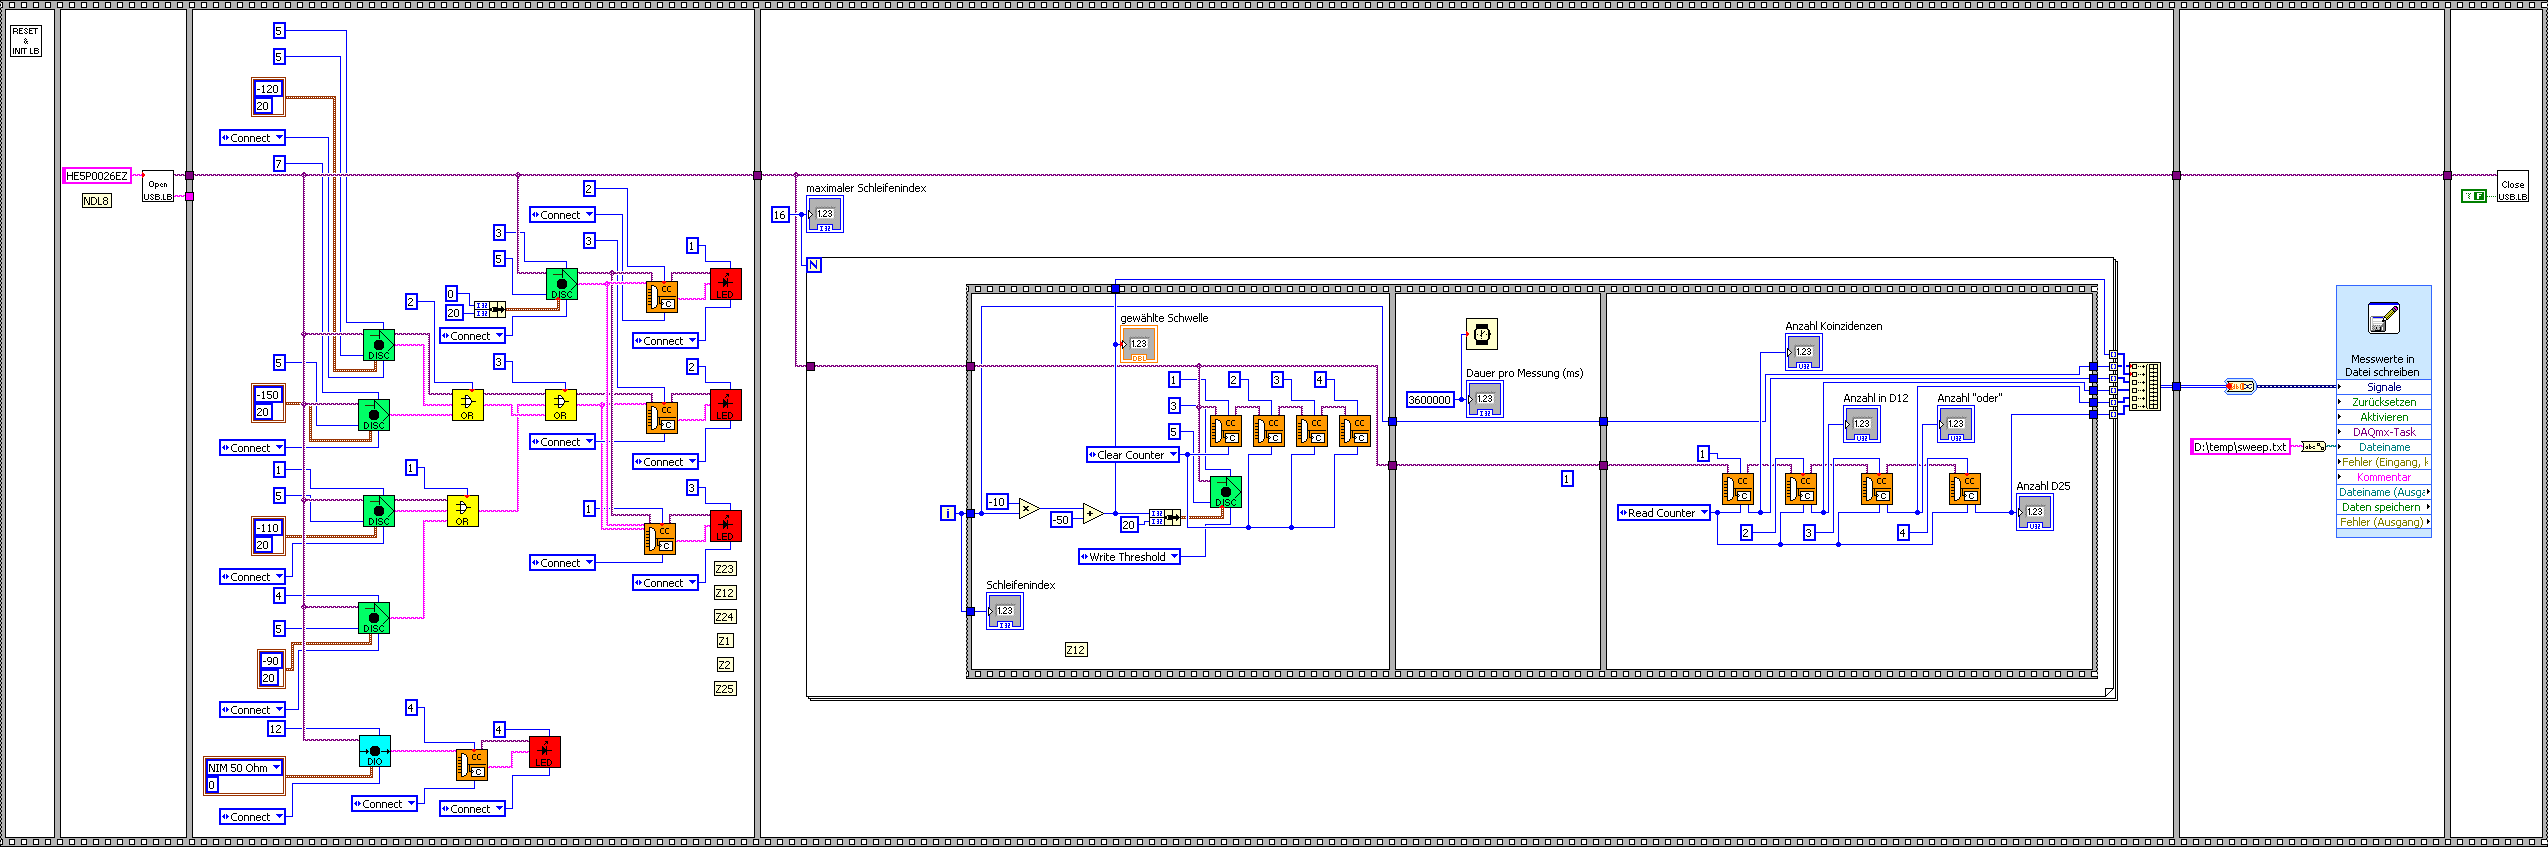
\includegraphics[width=\linewidth]{../Programm_kombiniert.png}
        \caption{%
            Das von uns entwickelte LabVIEW Programm zur Schwellenbestimmung.
            Es geht verschiedene Schwellenwerte durch, nimmt für eine feste
            Zeit Ereignisse auf und speichert die Resultate in einer Datei.
        }
        \label{fig:labview-programm}
    \end{figure}
\end{landscape}

\subsubsection{Auswertung der Daten}

Die Daten, die über Nacht durch das LabVIEW Programm gemessen worden sind, sind
in Tabelle~\ref{tab:winkel-daten} aufgelistet. In
Abbildung~\ref{fig:winkel-koinzidenz} ist die Anzahl der Koinzidenzen gegen die
eingestellte Schwelle zusammen mit der ersten Ableitung dargestellt.

\begin{figure}[htbp]
    \centering
    \tikzsetnextfilename{winkel-koinzidenz}
    \begin{tikzpicture}
        % let both axes use the same layers
        \pgfplotsset{set layers}
        \begin{axis}[
                %width=\linewidth,
                height=0.55\linewidth,
                scale only axis,
                grid=major,
                xmin=-210,
                xmax=-40,
                axis y line*=left,
                xlabel={Schwelle / \si{\milli\volt}},
                ylabel={Anzahl der Koinzidenzen},
            ]
            \addplot[
                black,
                only marks,
                mark=+,
                error bars/.cd,
                y dir=both,
                y explicit
            ] table[y error index=2] {winkel-schwelle-ratio.csv};
        \end{axis}
        \begin{axis}[
                height=0.55\linewidth,
                scale only axis,
                xmin=-210,
                xmax=-40,
                axis y line*=right,
                axis x line=none,
                ylabel={numerische Ableitung (rot)},
            ]
            \addplot[
                red,
                only marks,
                mark=+,
                error bars/.cd,
                y dir=both,
                y explicit
            ] table[y error index=2] {winkel-schwelle-steigung.csv};
        \end{axis}
    \end{tikzpicture}
    \caption{%
        Anzahl der Koinzidenzen gegen die eingestellte Schwelle. Zusätzlich ist
        in rot die numerische Ableitung eingetragen.
    }
    \label{fig:winkel-koinzidenz}
\end{figure}

Wir benutzen als Schwelle nun \SI{-125}{\milli\volt}, da dort das Minimum der
ersten Ableitung ist, es sich also um einen Wendepunkt in der gewünschten
Richtung handelt.

\subsection{Optimieren der Verzögerung}
\label{sec:optimieren_verzoegerung}

Das LabVIEW Programm, das für die Langzeitmessung benutzt wird, ist so
aufgebaut, dass auf einem der Digitalausgänge der NIMBox das Signal von D12
liegt. Dieses wird durch einen Gate Delay Generator verlängert und dient als
Gatesignal für den MCA. Das analoge Signal von Z12 wird in einem
Shapingamplifier derart umgeformt, dass es positiv ist und eine mit dem MCA
kompatible Form hat. Dieses Signal wird noch verzögert, damit es sich mit dem
Gatesignal aus der NIMBox überschneidet.

Diese Überschneidung haben wir auf dem Oszilloskop betrachtet. Aufgrund der
geringen Ereignisrate sind wir im Einzelschrittmodus vorgegangen. Da ein
einzelnes Oszillogramm mit Überlappung nicht viel aussagt, haben wir einige Bilder
gespeichert. Auf alle diesen ist die Überlappung gut, so dass die Verzögerung,
die bereits eingestellt war, korrekt ist. Dies ist in
Abbildung~\ref{fig:koinzidenz} abgebildet.

\begin{figure}[htbp]
    \centering
    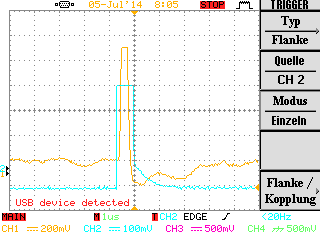
\includegraphics[width=0.47\linewidth]{../Daten/DS0000.png}
    \hfill
    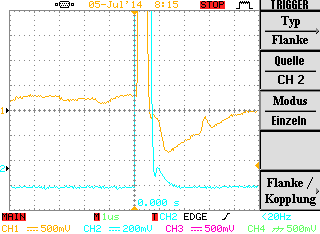
\includegraphics[width=0.47\linewidth]{../Daten/DS0002.png}

    \vspace*{5ex}

    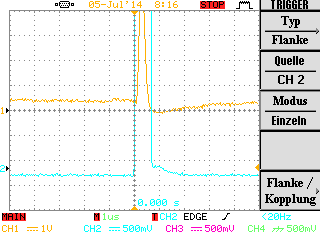
\includegraphics[width=0.47\linewidth]{../Daten/DS0003.png}
    \caption{%
        Oszillogramme zur Koinzidenz vom analogen Z12 Signal gegen das
        dazugehörige Gatesignal. Auf Kanal~1 (orange) ist das analoge Signal
        von Z12, auf Kanal~2 (cyan) das Gatesignal. Der Trigger liegt auf der
        steigenden Flanke auf Kanal~2.
    }
    \label{fig:koinzidenz}
\end{figure}

\section{Langzeitmessung zur Winkelverteilung}
\label{sec:langzeit_winkel}

\begin{figure}[htbp]
    \centering
    \tikzsetnextfilename{winkel-fit}
    \begin{tikzpicture}
        \begin{axis}[
                width=\linewidth,
                height=0.55\linewidth,
                grid=major,
                xlabel={Winkel / \si\degree},
                ylabel={Anzahl},
            ]
            \addplot[
                black,
                only marks,
                mark=+,
                error bars/.cd,
                y dir=both,
                y explicit
            ] table[y error index=2] {winkel-daten.csv};
            \addplot[red] table {winkel-fit.csv};
        \end{axis}
    \end{tikzpicture}
    \caption{%
    }
    \label{fig:winkel-fit}
\end{figure}

\section{Langzeitmessung des Pulshöhenspektrums}
\label{sec:langzeit_puls}

\chapter{Myonenlebensdauer}

\section{Aufbau}

\subsection{Detektoren}

Da wir eine Lebensdauer messen möchten, brauchen wir zwei Detektoren. Wir
benutzen hier einen schmalen über einer hohen Detektor. Beide sind unter einer
\SI{5}{\centi\meter} dicken Bleiabschirmung angebracht, um nur die harte
Komponente der Höhenstrahlung durchzulassen.

Der obere und untere Detektor liefert uns, sofern sie gleichzeitig aktiviert
werden, ein Startsignal für die Lebensdauermessung. Der untere Detektor gibt
das dazugehörige \textsc{Stop}-Signal.

Die Beschaltung ist in Abbildung~\ref{fig:aufbau-muon} gezeigt.

% TODO Vielleicht hier noch ein Bild zum Aufbau?

\subsection{Monitorkreis}

Zur Einstellung der Diskriminatorschwelle und der benötigten Verzögerung
zwischen Start- und Stop-Signal müssten wir Schwellen- und Verzögerungskurven
aufnehmen. Jedoch sind die Zählraten so gering, dass wir keine sinnvollen
Aussagen treffen können.

Daher bauen wir die Elektronik ein zweites Mal auf, lassen allerdings
Schwellenwerte und Verzögerungen unverändert. Unsere Messgröße sind dann die
Zählratenverhältnisse der beiden Kreise. Mit dieser ist eine sinnvolle
Einstellung der Diskriminatorschwellen möglich.

Nachdem alles eingestellt ist, wird dieser Kreis nicht mehr benötigt.

\begin{figure}[htbp]
    \centering
    \tikzsetnextfilename{aufbau-muon}
    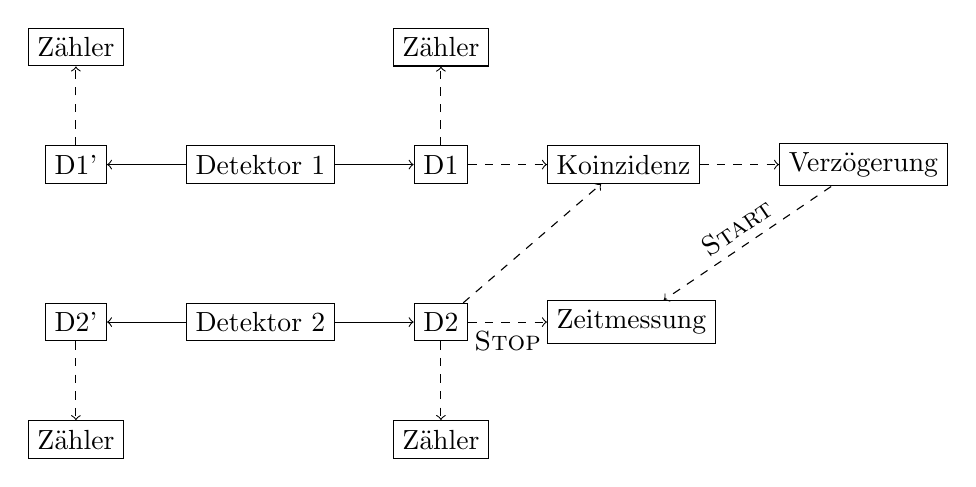
\begin{tikzpicture}
        \node[draw, rectangle] (Z1) at (0, 0) {Detektor 1};
        \node[draw, rectangle] (Z2) at (0, -2) {Detektor 2};

        \node[draw, rectangle, right=of Z1] (D1) {D1};
        \node[draw, rectangle, right=of Z2] (D2) {D2};

        \node[draw, rectangle, left=of Z1] (D1x) {D1'};
        \node[draw, rectangle, left=of Z2] (D2x) {D2'};

        \node[draw, rectangle, right=of D1] (K1) {Koinzidenz};
        \node[draw, rectangle, right=of K1] (V1) {Verzögerung};

        \node[draw, rectangle, right=of D2] (Zeit1) {Zeitmessung};

        \node[draw, rectangle, above=of D1] (Zahl1) {Zähler};
        \node[draw, rectangle, above=of D1x] (Zahl1x) {Zähler};
        \node[draw, rectangle, below=of D2] (Zahl2) {Zähler};
        \node[draw, rectangle, below=of D2x] (Zahl2x) {Zähler};

        \draw[->] (Z1) -- (D1);
        \draw[->] (Z2) -- (D2);
        \draw[->] (Z1) -- (D1x);
        \draw[->] (Z2) -- (D2x);

        \begin{scope}[dashed]
            \draw[->] (D1) -- (K1);
            \draw[->] (D2) -- (K1);
            \draw[->] (K1) -- (V1);
            \draw[->] (V1) -- (Zeit1) node[midway, sloped, above] {\textsc{Start}};
            \draw[->] (D2) -- (Zeit1) node[midway, sloped, below] {\textsc{Stop}};
            \draw[->] (D1) -- (Zahl1);
            \draw[->] (D2) -- (Zahl2);
            \draw[->] (D1x) -- (Zahl1x);
            \draw[->] (D2x) -- (Zahl2x);
        \end{scope}
    \end{tikzpicture}
    \caption{%
        Aufbau mit Monitorkreis (links) und Kreis zur Zeitmessung (rechts). Die
        „D“ bezeichnen die Diskriminatoren. Analoge Signale sind durch
        durchgezogene Linien gekennzeichnet, Digitale durch Gestrichelte.
    }
    \label{fig:aufbau-muon}
\end{figure}

\subsection{Zeitmessung}

Für die Zeitmessung benutzen wir die Pulse eines \SI{20}{\mega\hertz}
Oszillators. Nach dem Startsignal werden die Pulse gezählt. Die Länge einer
Periode sind \SI{50}{\nano\second}. Diese werden mit $1:20$-Untersetzern
auf eine größere Periode umgewandelt.

Zehn Sichtzähler erstellen eine Art Histogram mit Intervallgröße
\SI{1}{\micro\second}. Für den Fall, dass innerhalb der \SI{10}{\micro\second},
die dargestellt werden können, kein \textsc{Stop}-Impuls kommt, wird das
dahinter liegende Zählwerk zurückgesetzt. Somit ist die Totzeit durch ein
Zufallsimpuls oder ein sehr langlebiges Myon begrenzt.

Der \textsc{Stop}-Impuls löst außerdem eine Sperre für das
\textsc{Start}-Signal aus, damit der passende Sichtzähler um eins erhöht werden
kann. Und damit das keine unnötige Totzeit generiert, wenn die
\SI{10}{\micro\second} abgelaufen sind, wird durch den letzten Zähler ein
weiterer Impuls erzeugt, der die Sperre wieder außer Kraft setzt.

\section{Durchführung}

\subsection{Aufbau der Elektronik}

% TODO

\subsection{Aufnahme der Schwellenkurve}

Wir stellen die Diskriminatorschwellen des Monitorkreises auf das Minimum. Dann
gehen wir per Hand die Diskriminatorschwellen für den Messkreis durch und
messen die Anzahl der Ereignisse, die in \SI{600}{\second} eintreffen. Die
rohen Messdaten sind in Tabelle~\ref{tab:schwellen_roh}.

Für uns interessant ist das Verhältnis der Zählraten von Mess- und
Monitorkreis. Diese sind für den ersten Detektor in
Tabelle~\ref{tab:table_ratio_c1} aufgelistet und in
Abbildung~\ref{fig:ratio-data-c1} dargestellt. Um den Wendepunkt ablesen zu
können, haben wir die numerische Ableitung gebildet und ebenfalls in das
Diagramm eingetragen.

\begin{figure}[htbp]
    \centering
    \tikzsetnextfilename{ratio-data-c1}
    \begin{tikzpicture}
        % let both axes use the same layers
        \pgfplotsset{set layers}
        \begin{axis}[
                %width=\linewidth,
                height=0.55\linewidth,
                scale only axis,
                grid=major,
                xmin=-2.2,
                xmax=-0.4,
                axis y line*=left,
                xlabel={Schwelle / \si\volt},
                ylabel={Verhältnis der Zählraten},
            ]
            \addplot[
                black,
                only marks,
                mark=+,
                error bars/.cd,
                y dir=both,
                y explicit
            ] table[y error index=2] {ratio-data-c1.csv};
        \end{axis}
        \begin{axis}[
                height=0.55\linewidth,
                scale only axis,
                xmin=-2.2,
                xmax=-0.4,
                axis y line*=right,
                axis x line=none,
                ylabel={numerische Ableitung (rot)},
            ]
            \addplot[
                red,
                only marks,
                mark=+,
                error bars/.cd,
                y dir=both,
                y explicit
            ] table[y error index=2] {ratio-diff-c1.csv};
        \end{axis}
    \end{tikzpicture}
    \caption{%
        Verhältnis der Zählraten von Mess- und Monitorkreis des ersten
        Detektors. Zusätzlich ist in rot die numerische Ableitung eingetragen.
    }
    \label{fig:ratio-data-c1}
\end{figure}

Aus diesen Daten haben wir eine Schwelle von \SI{-1.0}{\volt} abgelesen.

Für den zweiten Detektor sind wir analog vorgegangen. Die Verhältnisse sind in
Tabelle~\ref{tab:table_ratio_c2} aufgelistet und in
Abbildung~\ref{fig:ratio-data-c2} dargestellt.

\begin{figure}[htbp]
    \centering
    \tikzsetnextfilename{ratio-data-c2}
    \begin{tikzpicture}
        % let both axes use the same layers
        \pgfplotsset{set layers}
        \begin{axis}[
                %width=\linewidth,
                height=0.55\linewidth,
                scale only axis,
                grid=major,
                axis y line*=left,
                xmin=-2.2,
                xmax=-0.4,
                xlabel={Schwelle / \si\volt},
                ylabel={Verhältnis der Zählraten},
            ]
            \addplot[
                black,
                only marks,
                mark=+,
                error bars/.cd,
                y dir=both,
                y explicit
            ] table[y error index=2] {ratio-data-c2.csv};
        \end{axis}
        \begin{axis}[
                height=0.55\linewidth,
                scale only axis,
                axis y line*=right,
                xmin=-2.2,
                xmax=-0.4,
                axis x line=none,
                ylabel={numerische Ableitung (rot)},
            ]
            \addplot[
                red,
                only marks,
                mark=+,
                error bars/.cd,
                y dir=both,
                y explicit
            ] table[y error index=2] {ratio-diff-c2.csv};
        \end{axis}
    \end{tikzpicture}
    \caption{%
        Verhältnis der Zählraten von Mess- und Monitorkreis des ersten
        Detektors. Zusätzlich ist in rot die numerische Ableitung eingetragen.
    }
    \label{fig:ratio-data-c2}
\end{figure}

Aus diesen Daten lesen wir \SI{-0.9}{\volt} als sinnvolle Schwelle ab.

\subsection{Einstellen der Verzögerung}

Das Signal aus der Koinzidenz der beiden Diskriminatoren schließen wir an die
beiden Verzögerungskabelspulen an, die am Schrank angebracht sind. Auf diese
Weise erhalten wir eine ausreichende Verzögerung des \textsc{Start}-Signals.

\subsection{Aufnahme der Lebensdauerkurve}

Das Verzögerungskabel schließen wir an den \textsc{Start}-Eingang des
Zeitmessers an, das Signal von Detektor~2 schließen wir an den
\textsc{Stop}-Eingang an. Wir setzen die 10 Sichtzähler zurück und lassen die
Messung die nächsten Tage laufen.

\section{Auswertung}

% TODO

\chapter{Ergebnis}

% TODO

\begin{appendix}
    \chapter{Rohe Messdaten}

    \section{Schwellenkurve Winkelverteilung}

    \begin{table}[htbp]
        \centering
        \begin{tabular}{*2S|*4S}
            {Index} &
            {Schwelle} &
            {Koinzidenzen} &
            {D12} &
            {oder} &
            {D25} \\
            \midrule
            %< for row in winkel_sweep_roh: >%
            << ' & '.join(row) >> \\
            %< endfor >%
        \end{tabular}
        \caption{%
            Rohe Messdaten von unserem LabVIEW Programm aus
            Abbildung~\ref{fig:labview-programm}.
        }
        \label{tab:winkel-daten}
    \end{table}

    \begin{landscape}
        \section{Schwellenkurve Myonlebensdauer}

        \begin{table}[htbp]
            \centering
            \begin{tabular}{*4S|*4S|S}
                {Me. 1} &
                {Me. 2} &
                {Mo. 1} &
                {Mo. 2} &
                {Me. 1} &
                {Me. 2} &
                {Mo. 1} &
                {Mo. 2} &
                {Zeit} \\
                \midrule
                %< for row in schwellen_roh: >%
                << ' & '.join(row) >> \\
                %< endfor >%
            \end{tabular}
            \caption{%
                Rohe Messdaten der Schwellenkurve für die Myonlebensdauer. Die
                ersten vier Spalten sind die Diskriminatorschwellen in
                \si\volt, wobei „Me“ für Mess- und „Mo“ für Monitorkreis steht.
                Die nächsten vier Spalten sind die Anzahl der Ereignisse. Die
                letzte Spalte ist die Zeit in \si\second.
            }
            \label{tab:schwellen_roh}
        \end{table}
    \end{landscape}

    \begin{table}[htbp]
        \centering
        \begin{tabular}{SS}
            {Diskriminatorschwelle / \si\volt} & {Verhältnis der Zählraten} \\
            \midrule
            %< for row in table_ratio_c1: >%
            << ' & '.join(row) >> \\
            %< endfor >%
        \end{tabular}
        \caption{%
            Diskriminatorschwellen und Verhältnis der Zählraten für den ersten
            Detektor.
        }
        \label{tab:table_ratio_c1}
    \end{table}

    \begin{table}[htbp]
        \centering
        \begin{tabular}{SS}
            {Diskriminatorschwelle / \si\volt} & {Verhältnis der Zählraten} \\
            \midrule
            %< for row in table_ratio_c2: >%
            << ' & '.join(row) >> \\
            %< endfor >%
        \end{tabular}
        \caption{%
            Diskriminatorschwellen und Verhältnis der Zählraten für den zweiten
            Detektor.
        }
        \label{tab:table_ratio_c2}
    \end{table}

\end{appendix}

\end{document}

% vim: spell spelllang=de tw=79
